% design.tex
\chapter{Design}
In this section of my NEA I will be including details on the detailed design of my Journal app. 


\section{Introduction}
The objective of my journal app is to provide users with an easily accessible and navigated app for digital journaling. To accomplish this, I will choose the Django REST framework for my backend server functionality and React, a powerful JavaScript library, for my frontend. In this section of my report I will be justifying why I have made these choices and detailing the specific designs for full stack application tailored to these frameworks

\section{Frontend}
Frontend primarily refers to the interface which the user interacts. The most common form of frontend is a webpage, which encompasses the layout and design elements of the website. Initially, webpages are created using HTML, CSS, and JavaScript. However, as time progresses, developers have devised ways to generate them. Using Python, for example, frameworks like Django and Flask allow developers to build HTML, CSS, and Javascript pages interactively and dynamically. In the case of Django and Flask, developers can use templating engines like Jinja2 to generate dynamic HTML pages by integrating Python code into the HTML layout, as well as being able to avoid boilerplate code by building templates for the layout of the appearance of the page and then being able to make changes to different pages while maintaining consistency across the website. This approach saves time since it lets me focus on the features instead of writing boilerplate code.

Behind the scenes, frontend is not only the UI, as it also includes the logic and functionality that drives the user experience. This includes handling user interactions, making API calls, data manipulation, and updating the UI based on user input.

Javascript frameworks are the most popular amongst web developers since there exist powerful libraries like React and Angular maintained by giant tech companies, and javascript is simply more widely adopted and used in the web development world. Similarly, I have heard good things about a library called Svelt, which offers a lightweight approach to building user interfaces. What I mean by that is it uses fewer codes, is truly reactive, and has no virtual DOM

Initially, I used Django to generate my frontend pages using its built-in templating engine dynamically. However, I want to create a more modular approach and, therefore, truly isolate my backend and frontend. The benefit of doing so is that I could connect a completely different front-end interface to the same backend functionality with ease via API communication. In my application, I will try my best to maintain the Single Responsibility design principle throughout my application development process.\\
To achieve achieve this modular approach, I decided to use a separate frontend to my Django backend, specifically React.js. React is the most popular and in-demand ecosystem developed by Facebook for building responsive user interfaces, Facebook developed React.js and later React native for building "truly native" mobile apps using JavaScript. React.js is the javascript library I chose for my web creation, and I believe that it would be a valuable learning experience to take on my first Javascript library to build my app.

\section{Backend}
Backend refers to the server side of a web application, where the logic behind the application is. It is responsible for processing requests, interacting with databases, and algorithmically generating responses to be sent back to the client and other background processes. There are frameworks available for different programming languages that can be used for backend development.

I have considered Python, C\# and Javascript frameworks for my project as I am proficient in Python, C\# (having dabbled with those in my own time and studied those languages for GCSE and A-Levels, respectively), and Javascript is a language I have always wanted to explore further since it is the most popular language; hence, there's wide support for it in terms of libraries and frameworks. Specifically, I have considered Django, FastAPI, Flask, Next.js, and ASP.NET Core frameworks.

\subsection{ASP.NET:}
ASP.NET is a powerful framework developed by Microsoft for building web apps and services using the .NET framework and C\#. It is capable and scalable, making it suitable for large-scale applications. Personally, however. I did not end up choosing ASP.NET due to my hardware constraint. I am running a MacOS unix system on the apple silicone architecture, which I could technically do .Net development using. However, from my experience in the past, it is a pain. In addition, ASP.NET was primarily suited for the Windows ecosystem (although they are trying to make it more platform-independent), meaning it is not optimal for me personally, and there are other better ways to create a university platform-independent backend.

\subsection{Next.js and Express.js:}
Two of the most demanding and powerful frameworks are these two are used to build the backend using Node.js. Next.js goes hand-in-hand with React since it provides server-side rendering. This is a thin client approach, where the initial HTML is generated on the server and then sent to the client. This approach ensures the smoothness of the user experience \cite{gillis_2020_fat}. Express.js is, on the other hand, a lightweight and flexible framework for building RESTful APIs and the like. It might be nice, but I am more comfortable with Python, so I decided that it's a good idea to only use Javascript for my Frontend development and Python for my Backend.

\subsection{Flask and FastAPI:}
Flask is a lightweight web framework for Python used to build APIs. I had previously dabbled with the framework and found it barebone and flexible. FastAPI is a much more modern alternative to Flask. It provides similar simplicity and flexibility but with the added benefit of high performance due to its asynchronous capabilities. I was really tempted to use FastAPI for my project, however, I had been learning a lot of Django and decided to go with it instead.

\subsection{Django}
Django is the most feature-rich mainstream backend web development framework in Python. It provides all the necessary tools I need, including URL routing, Database Object-Relational mapping, as well as overall security features preventing basic forms of attacks such as CSRF. This allows me to robustly build my application, focusing on functionalities that matter rather than reinventing the wheels. Django also allows me to have fine-tuned control over functionalities if I want to redesign, replace, or extend any parts. Even though Django might not be as performant as some other frameworks, such as FastAPI, it offers a well-established and stable platform for web development suitable for my Journal app.

\section{Hierarchy Charts}
Hierarchy charts are visual representations of a large problem being broken down into smaller components or sub-problems. They are charts in the form of an upside-down tree structure. Ideally, the problem should be broken down until each module is no longer than a page of code. In the charts I have created, I had to separate my application for two different charts. One for my Frontend and one for my Backend because the project is quite large. In the diagram, I have broken down my problems to a reasonably small size yet not too specific such that it becomes too difficult to maintain.

\subsection{Django Server Design:}
In this hierarchy chart, I have decomposed the design of my entire Django backend API into many smaller problems I will solve in my implementation. I will not be describing each individual problem in detail here. Still, the hierarchy chart provides a clear overview of how the different components and functionalities of the backend system are organised. See Figure \ref{fig:backendHD} for the chart.

\subsection{React Frontend}
In the hierarchy chart for the JavaScript frontend, I have broken down the design of my user interface and client-side functionalities into smaller components.

These components include user authentication, data retrieval from the backend API, the UI and more. In this chart, it's hard to show how the functions communicate at an inter-component level. However, on top of what's designed in the hierarchy chart, data is passed through props and the things under my state management box shown in the diagram would be accessible throughout my application by different components through the use of React Context and Context Provider. See Figure \ref{fig:frontendHD} for the chart.

\begin{landscape}
\begin{figure}
    \centering
    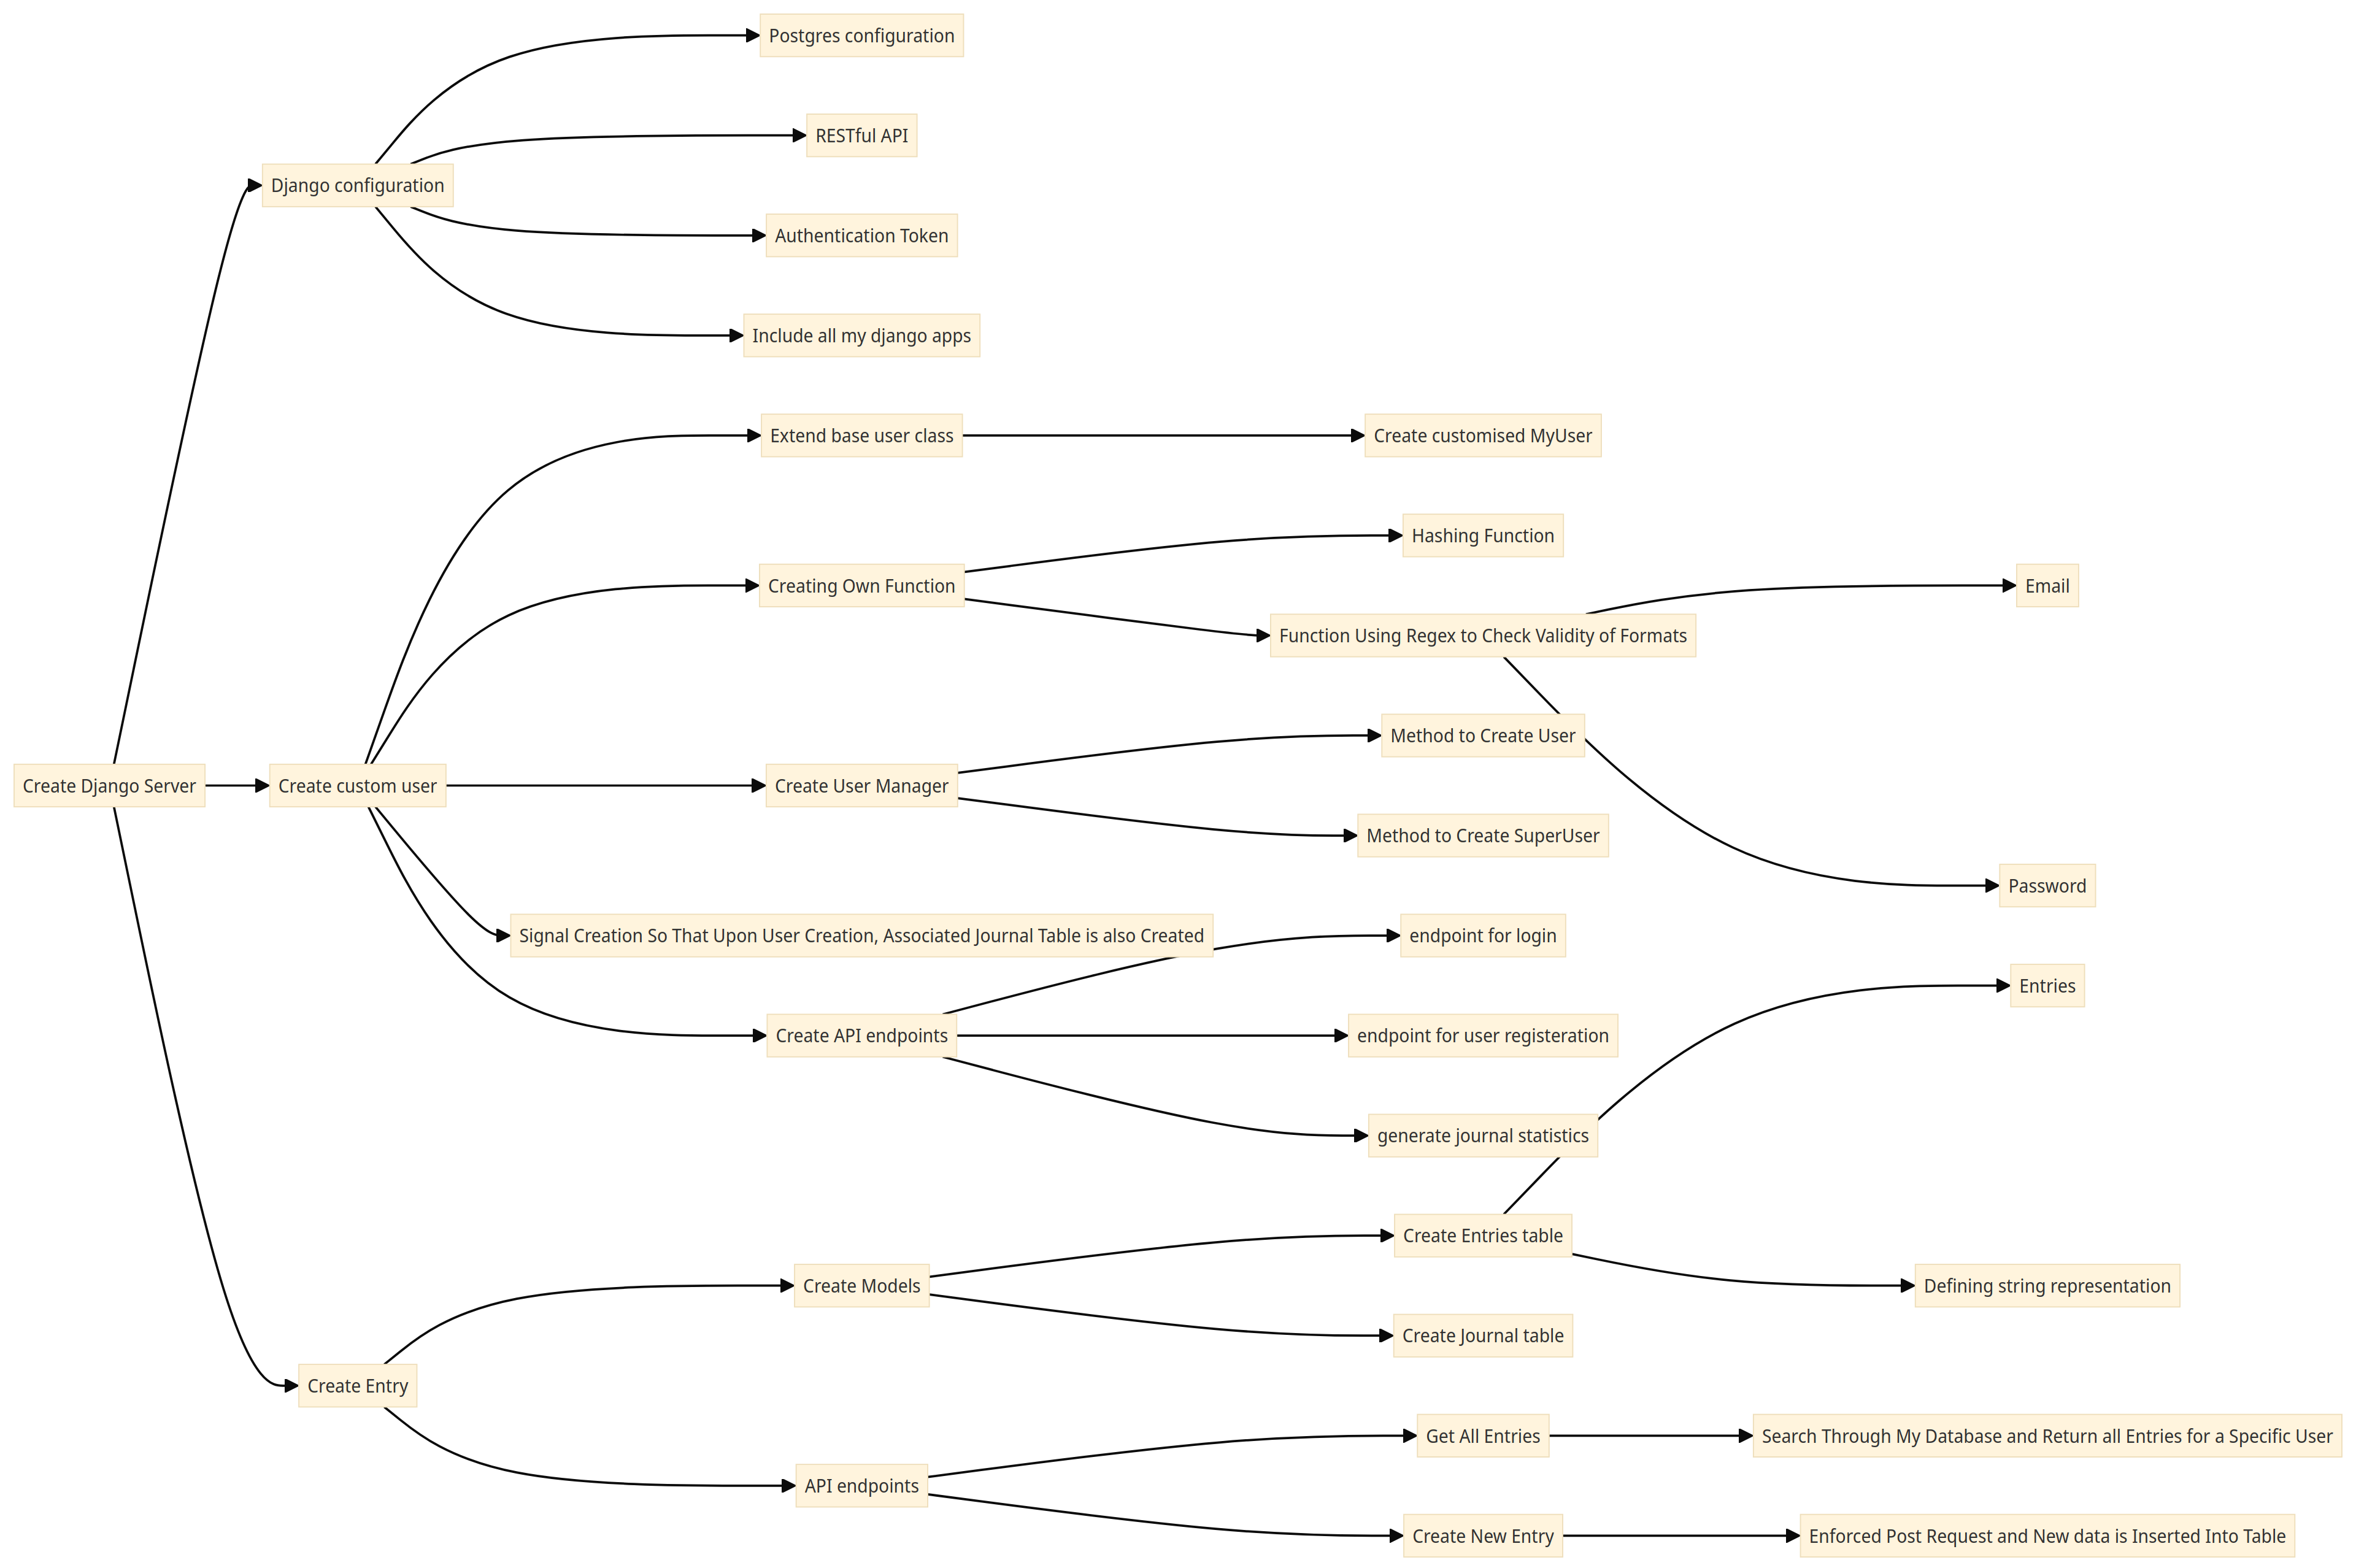
\includegraphics[
    width=1\linewidth,
    ]{Assets/Hierarchy_Backend.png}
    \caption{Backend Hierarchy Diagram}
    \label{fig:backendHD}
\end{figure}
\end{landscape}



\begin{landscape}
    \begin{figure}
        \centering
        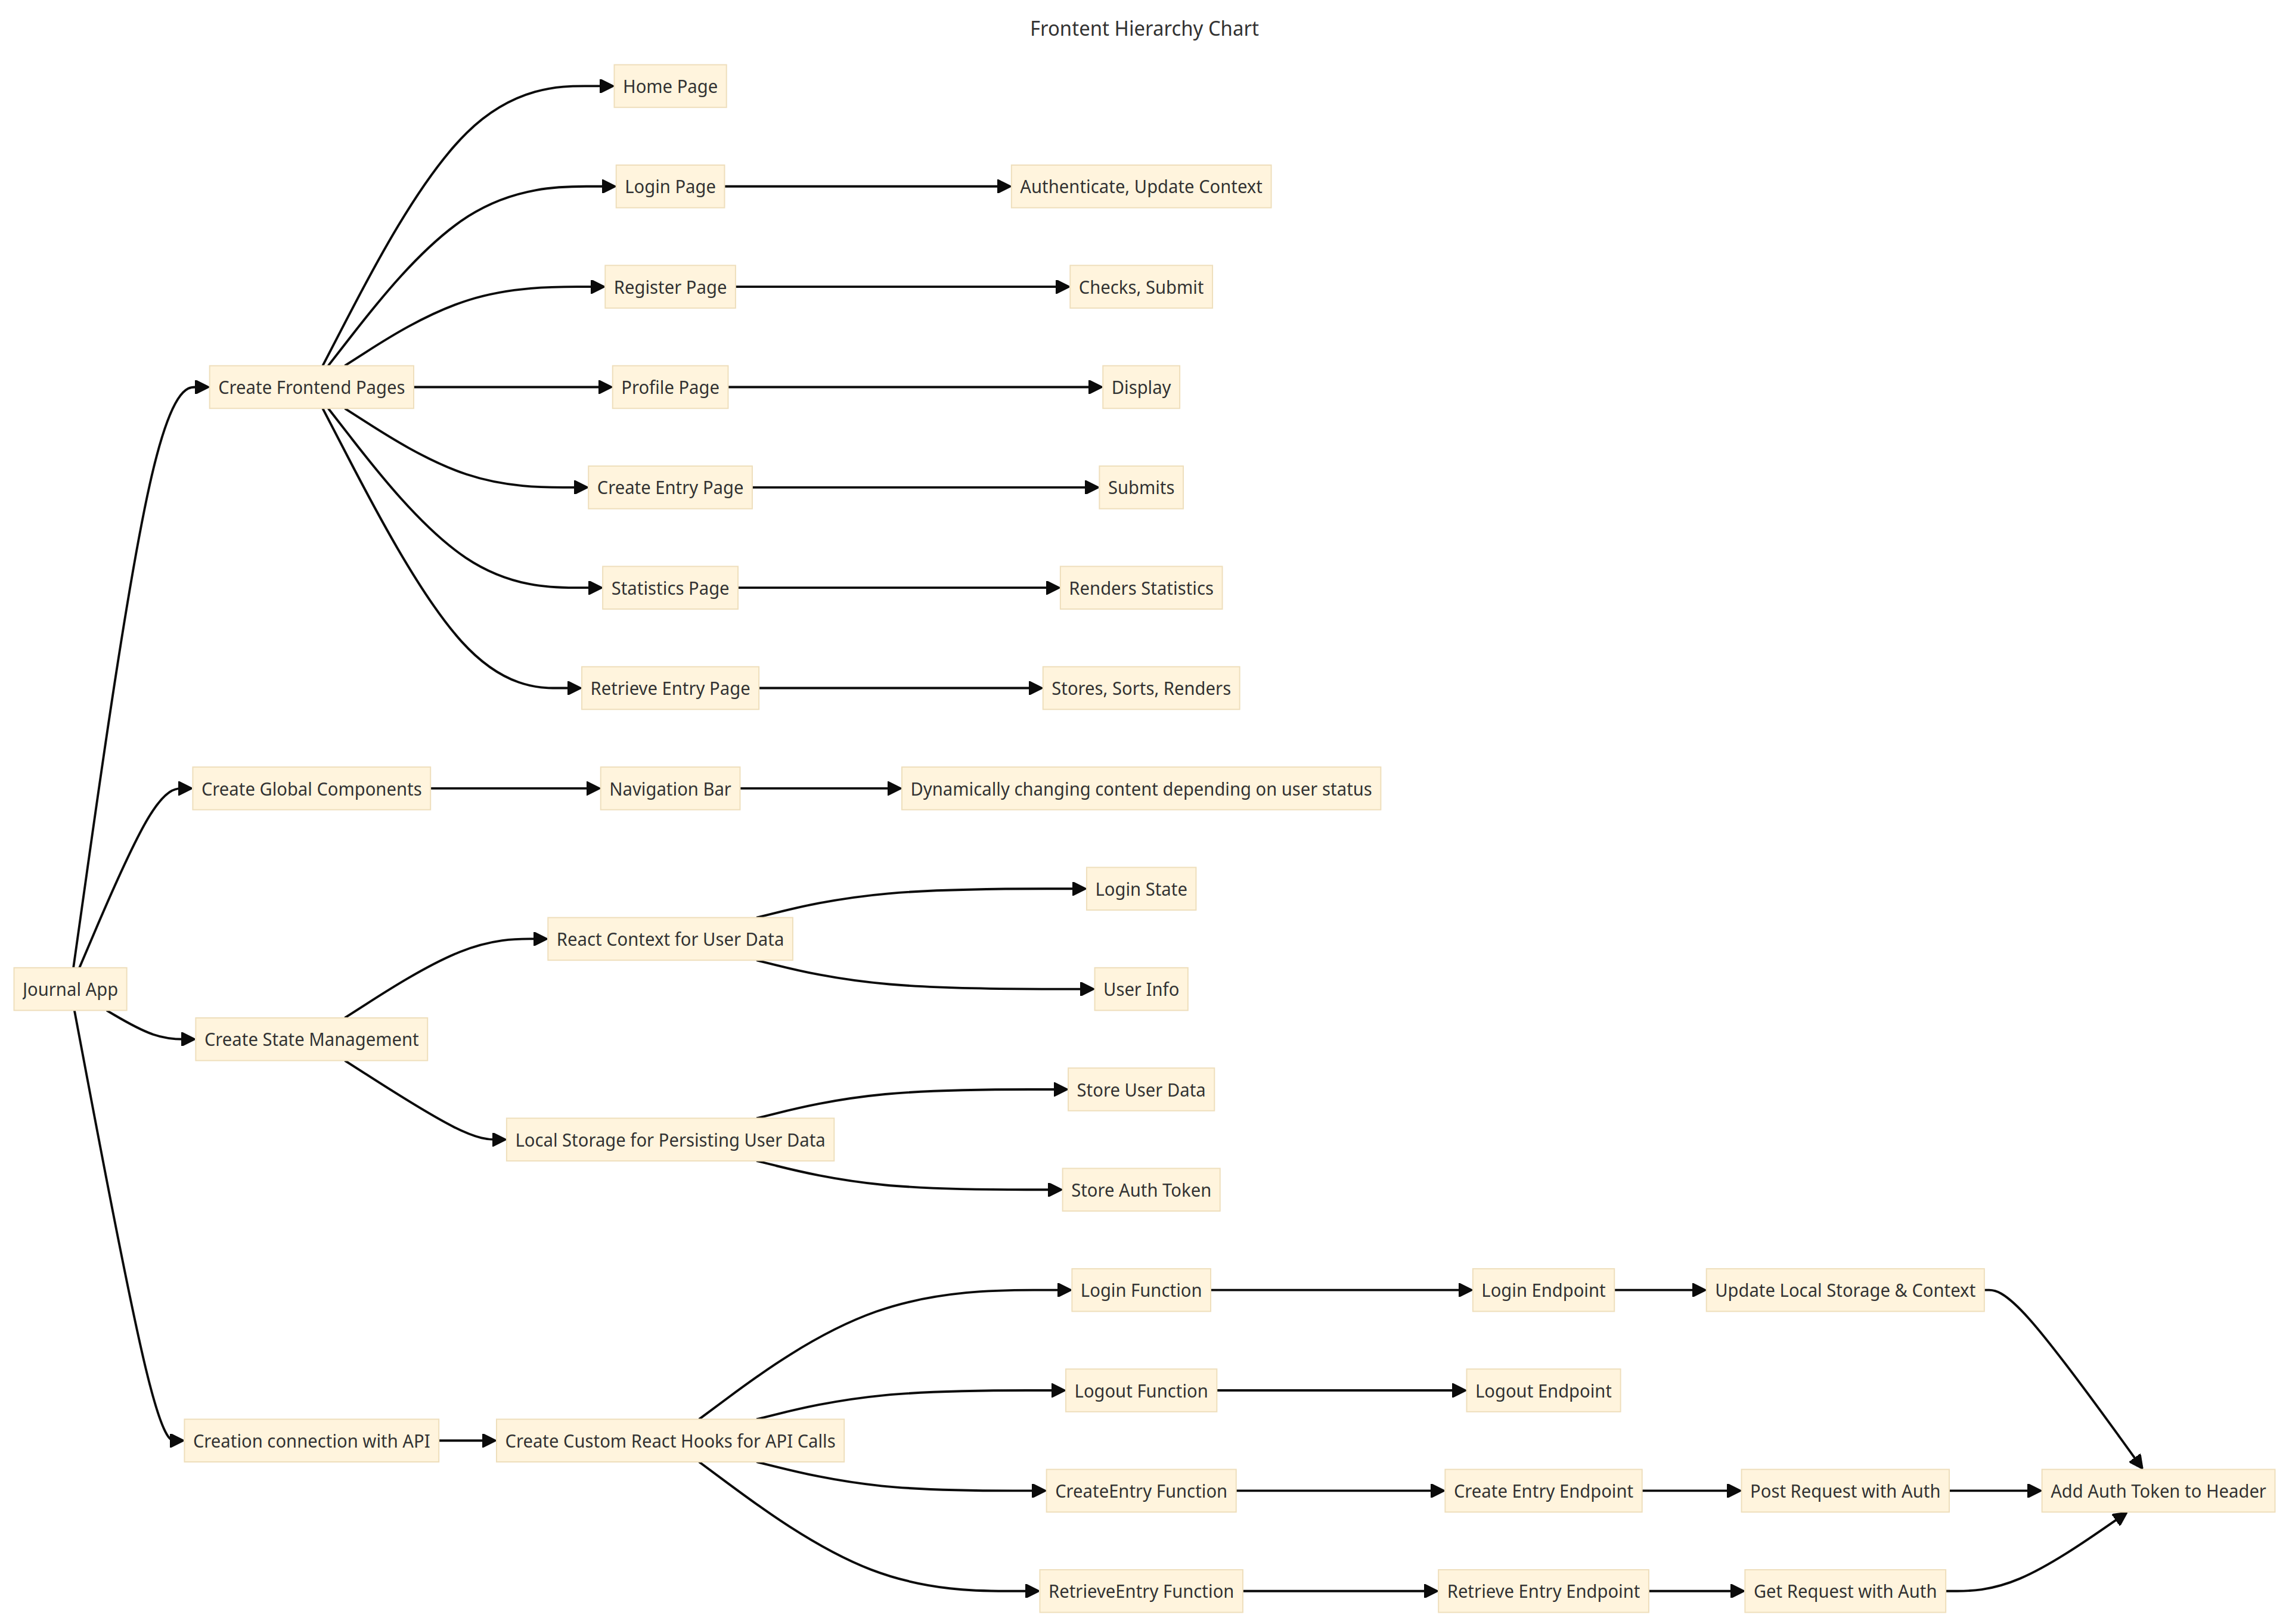
\includegraphics[width=1\linewidth]{Assets/FrontendER.png}
        \caption{Frontend Hierarchy Diagram}
        \label{fig:frontendHD}
    \end{figure}
\end{landscape}

\subsection{Flowchart}
Now, to bring everything together, I have designed a flowchart to depict the flow of operations across the entire system. The overall narrative of the flowchart is that the user interacts with the frontend web pages, and it would trigger functions in the frontend JavaScript code. These functions would perform operations such as making requests to the RESTful API endpoints exposed by the Backend or making changes to the storage in the browser. The front end also manipulates the storage system in the browser while the server handles the database. 

\begin{figure}[h]
    \centering
    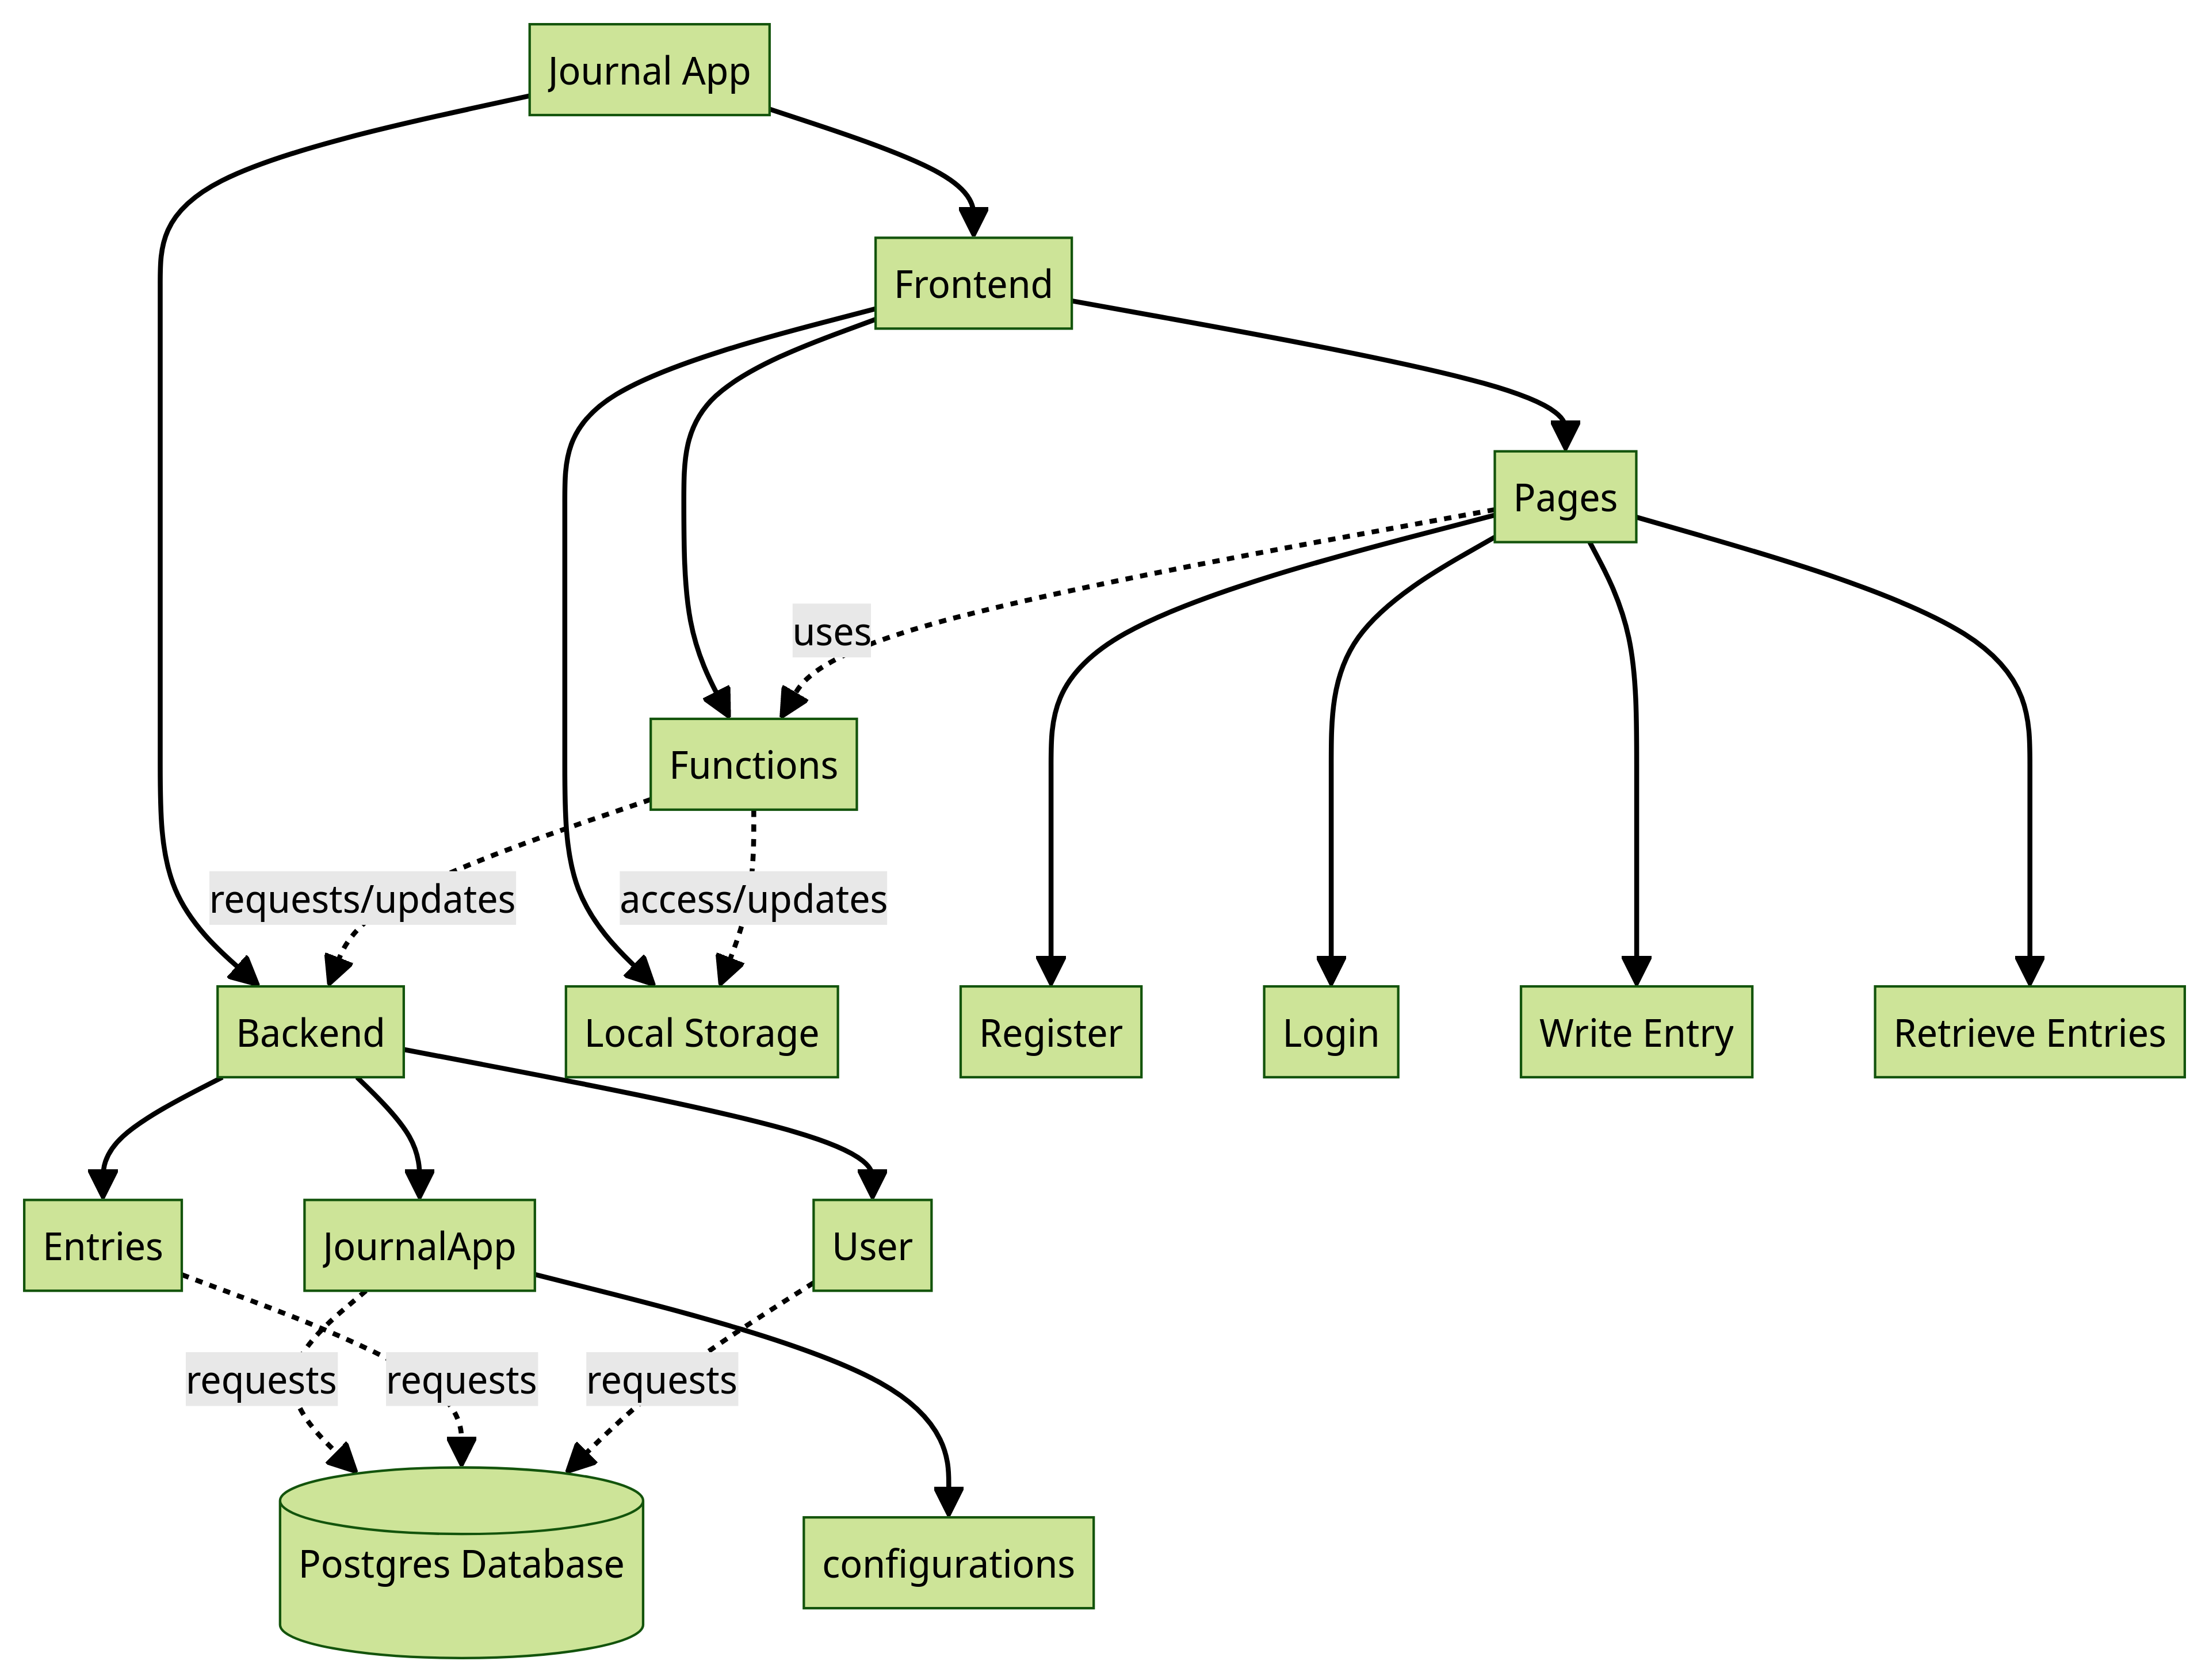
\includegraphics[width=5in]{Assets/Flowchart.png}
    \caption{Flowchart of the System}
    \label{fig:3.3}
\end{figure}



\section{Data Structures / Data Modelling}
\subsection{Entity Relationship Modelling}
\subsubsection{Storing Data}
In my application, data and the flow of data are integral to the system's overall functionality. I have decided to store the data centrally in a relational database. Central storage ensures reliability, scalability and ease of access of data for me. This is good for my users, who expect their data to be reliably stored and easily accessed.

While it is possible to implement a distributed data storage system for a journal app, I have chosen a centralised approach for simplicity and ease of implementation. Not only is a centralised database more accessible for amateur developers like myself but there are also other reasons why centralised storage is better for my journal app. Keeping entries in a structured place means opportunities to analyse the data. If the user opts in for these features, I could perform sentiment analysis on the user's entries or generate statistics and insights based on their journaling patterns. In fact, Google provides a model for analysing sentiment, which is easily accessible through their API. This is an additional thing I may implement after my project is complete.

I have chosen PostgreSQL as the database management system for my application. Postgres is the most powerful Open-Source option available, and once configured, it provides excellent support for my development environment.

Moreover, If I were to host my application, I could easily connect it to a Postgres database through a cloud provider like Railway.

Looking through the specifications of my journal app, I have identified data that needed to be stored and created a database design in the Third Normal Form.

\subsubsection{Entity Relationship Modelling}
\begin{figure}[!hbt]
    \centering
    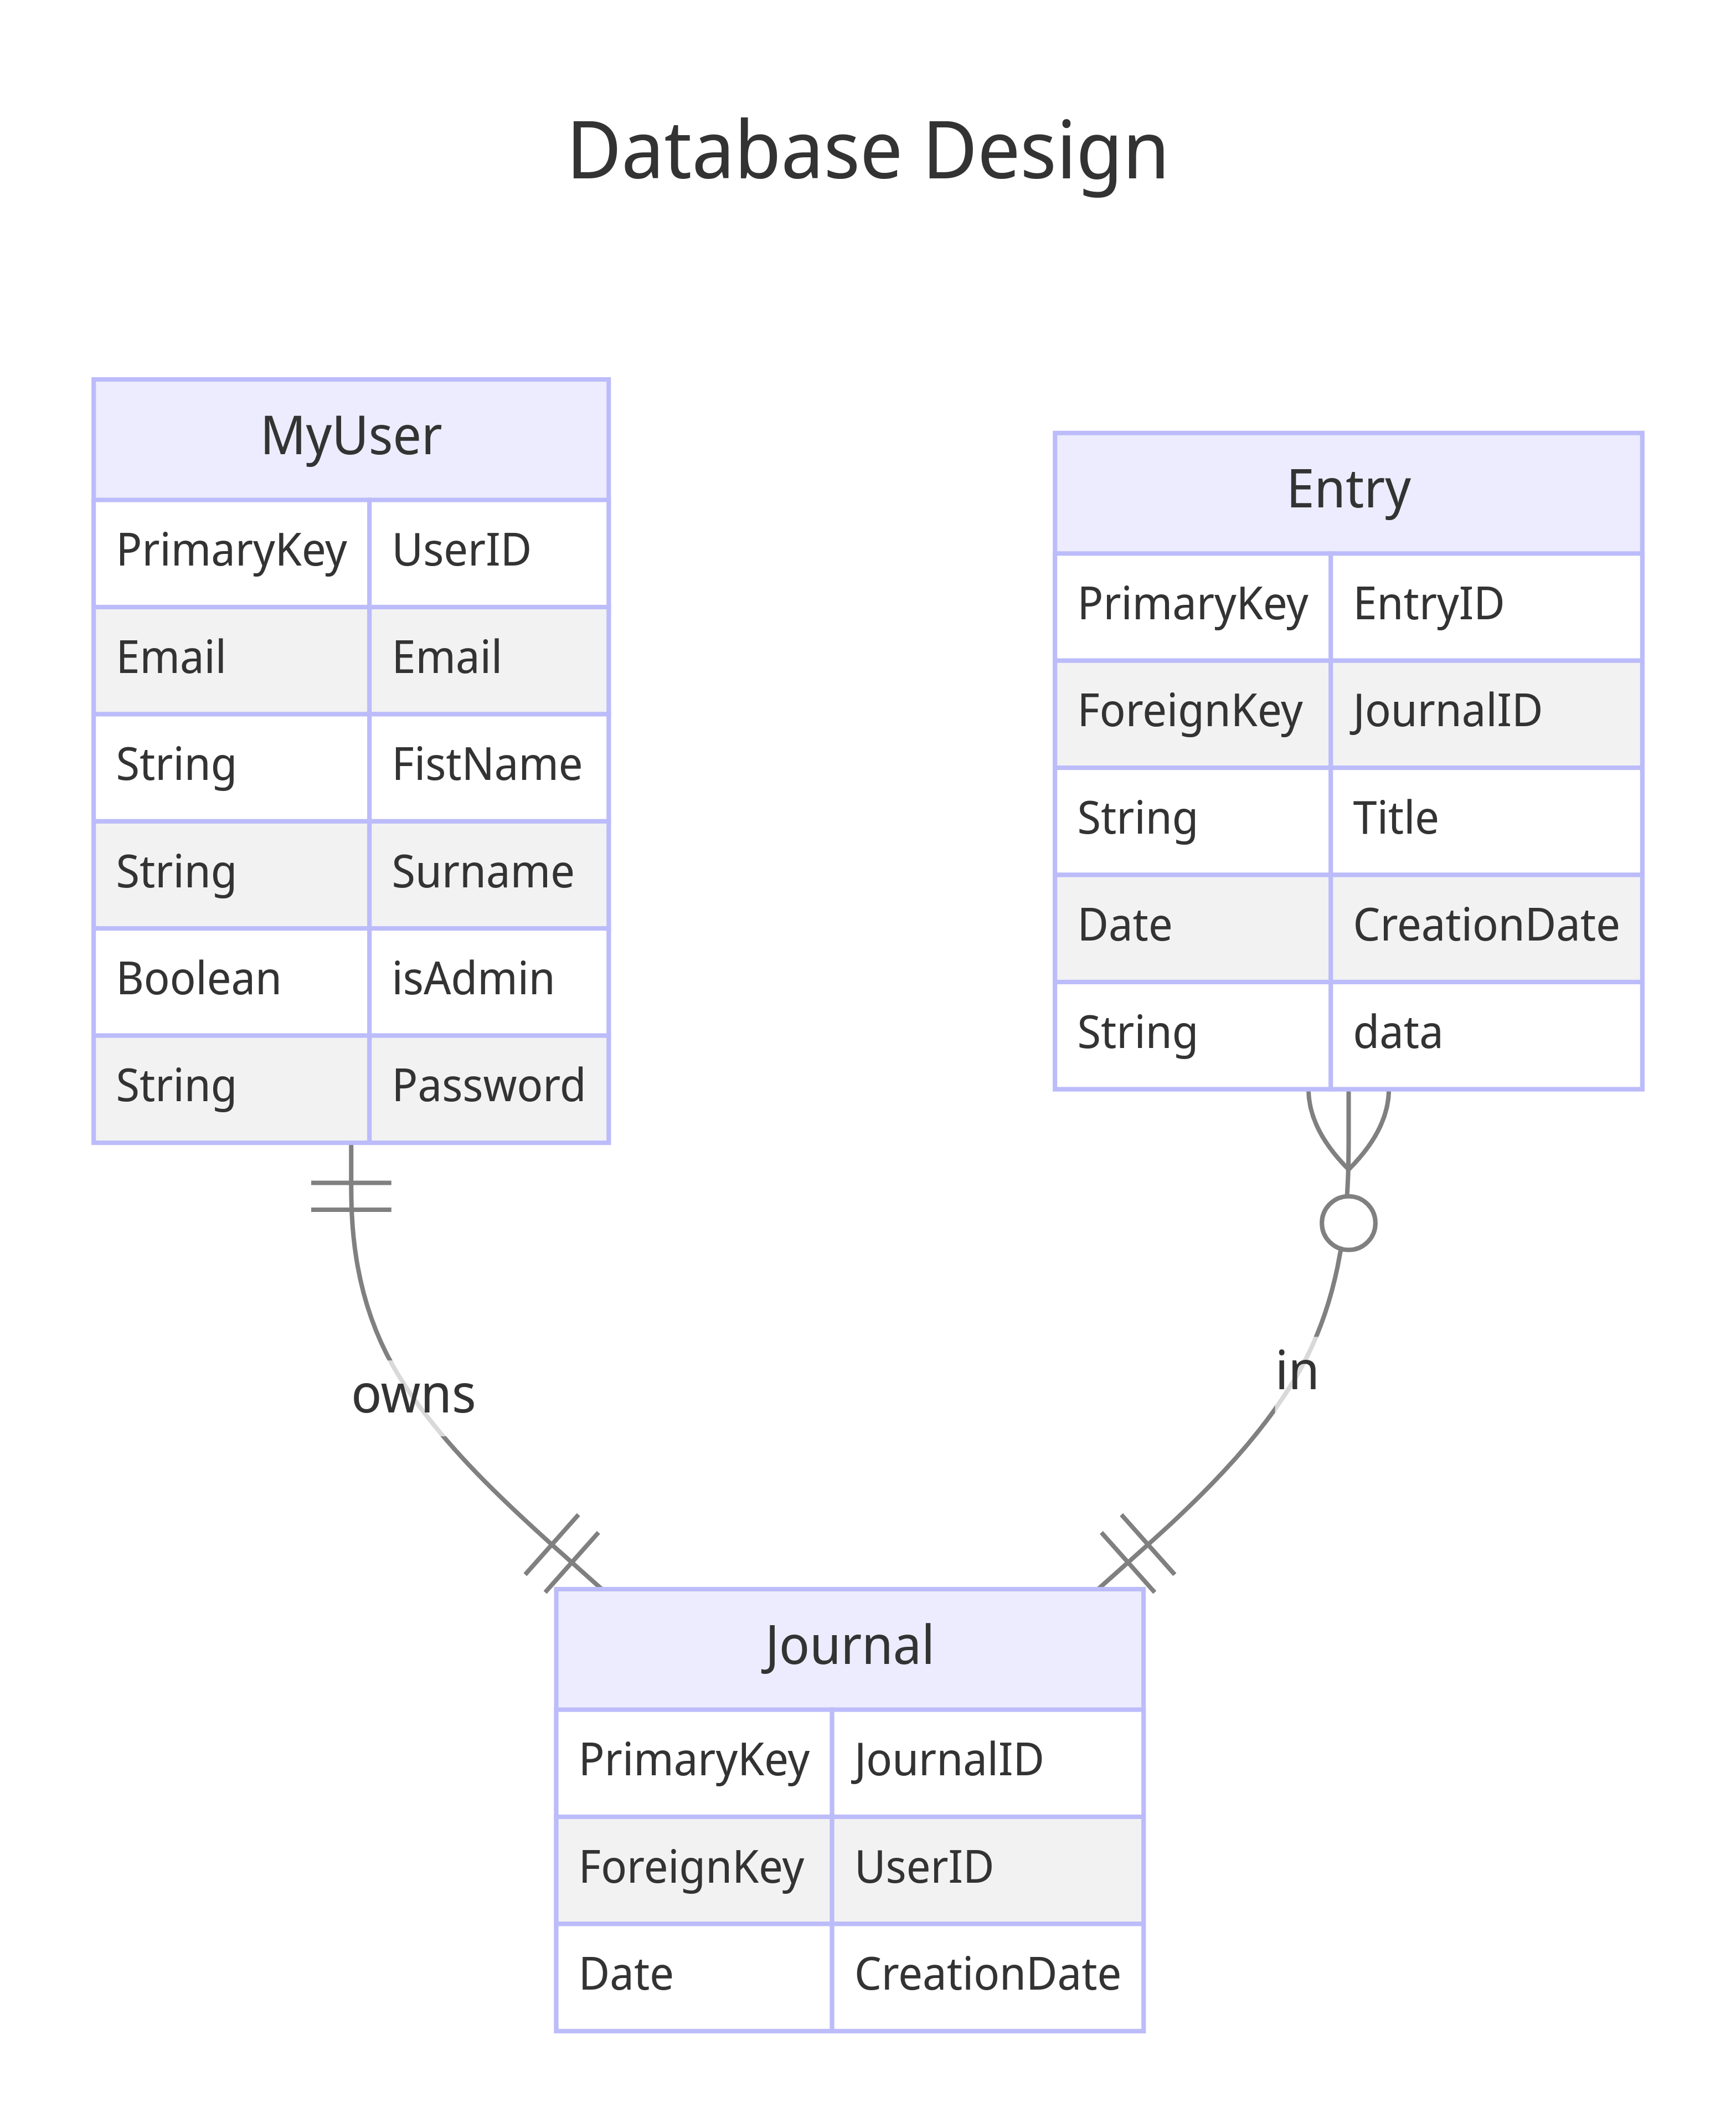
\includegraphics[width=\linewidth]{Assets/Journal Hierarchy ER diagram-2024-03-18-085346.png}
    \caption{Entity Relationship Diagram}
    \label{fig:ER}
\end{figure}


\subsection{Abstract Data Structures}



\subsection{External Data Sources}
Discuss any external data sources utilized.

\subsection{OOP Model}
One of the core features of Django is the built-in Object Relation Mapping, which enables me to Model my database using Objects. Initially, I explored writing SQL queries to create my database(see appendix), but as my project grew in complexity, I realised that to use some powerful features provided by Django, for example, the authentication and the administrator interface, it would be more efficient and convenient to use Django's Object Relation Mapping capabilities. 


\begin{figure}[!hbt]
    \centering
    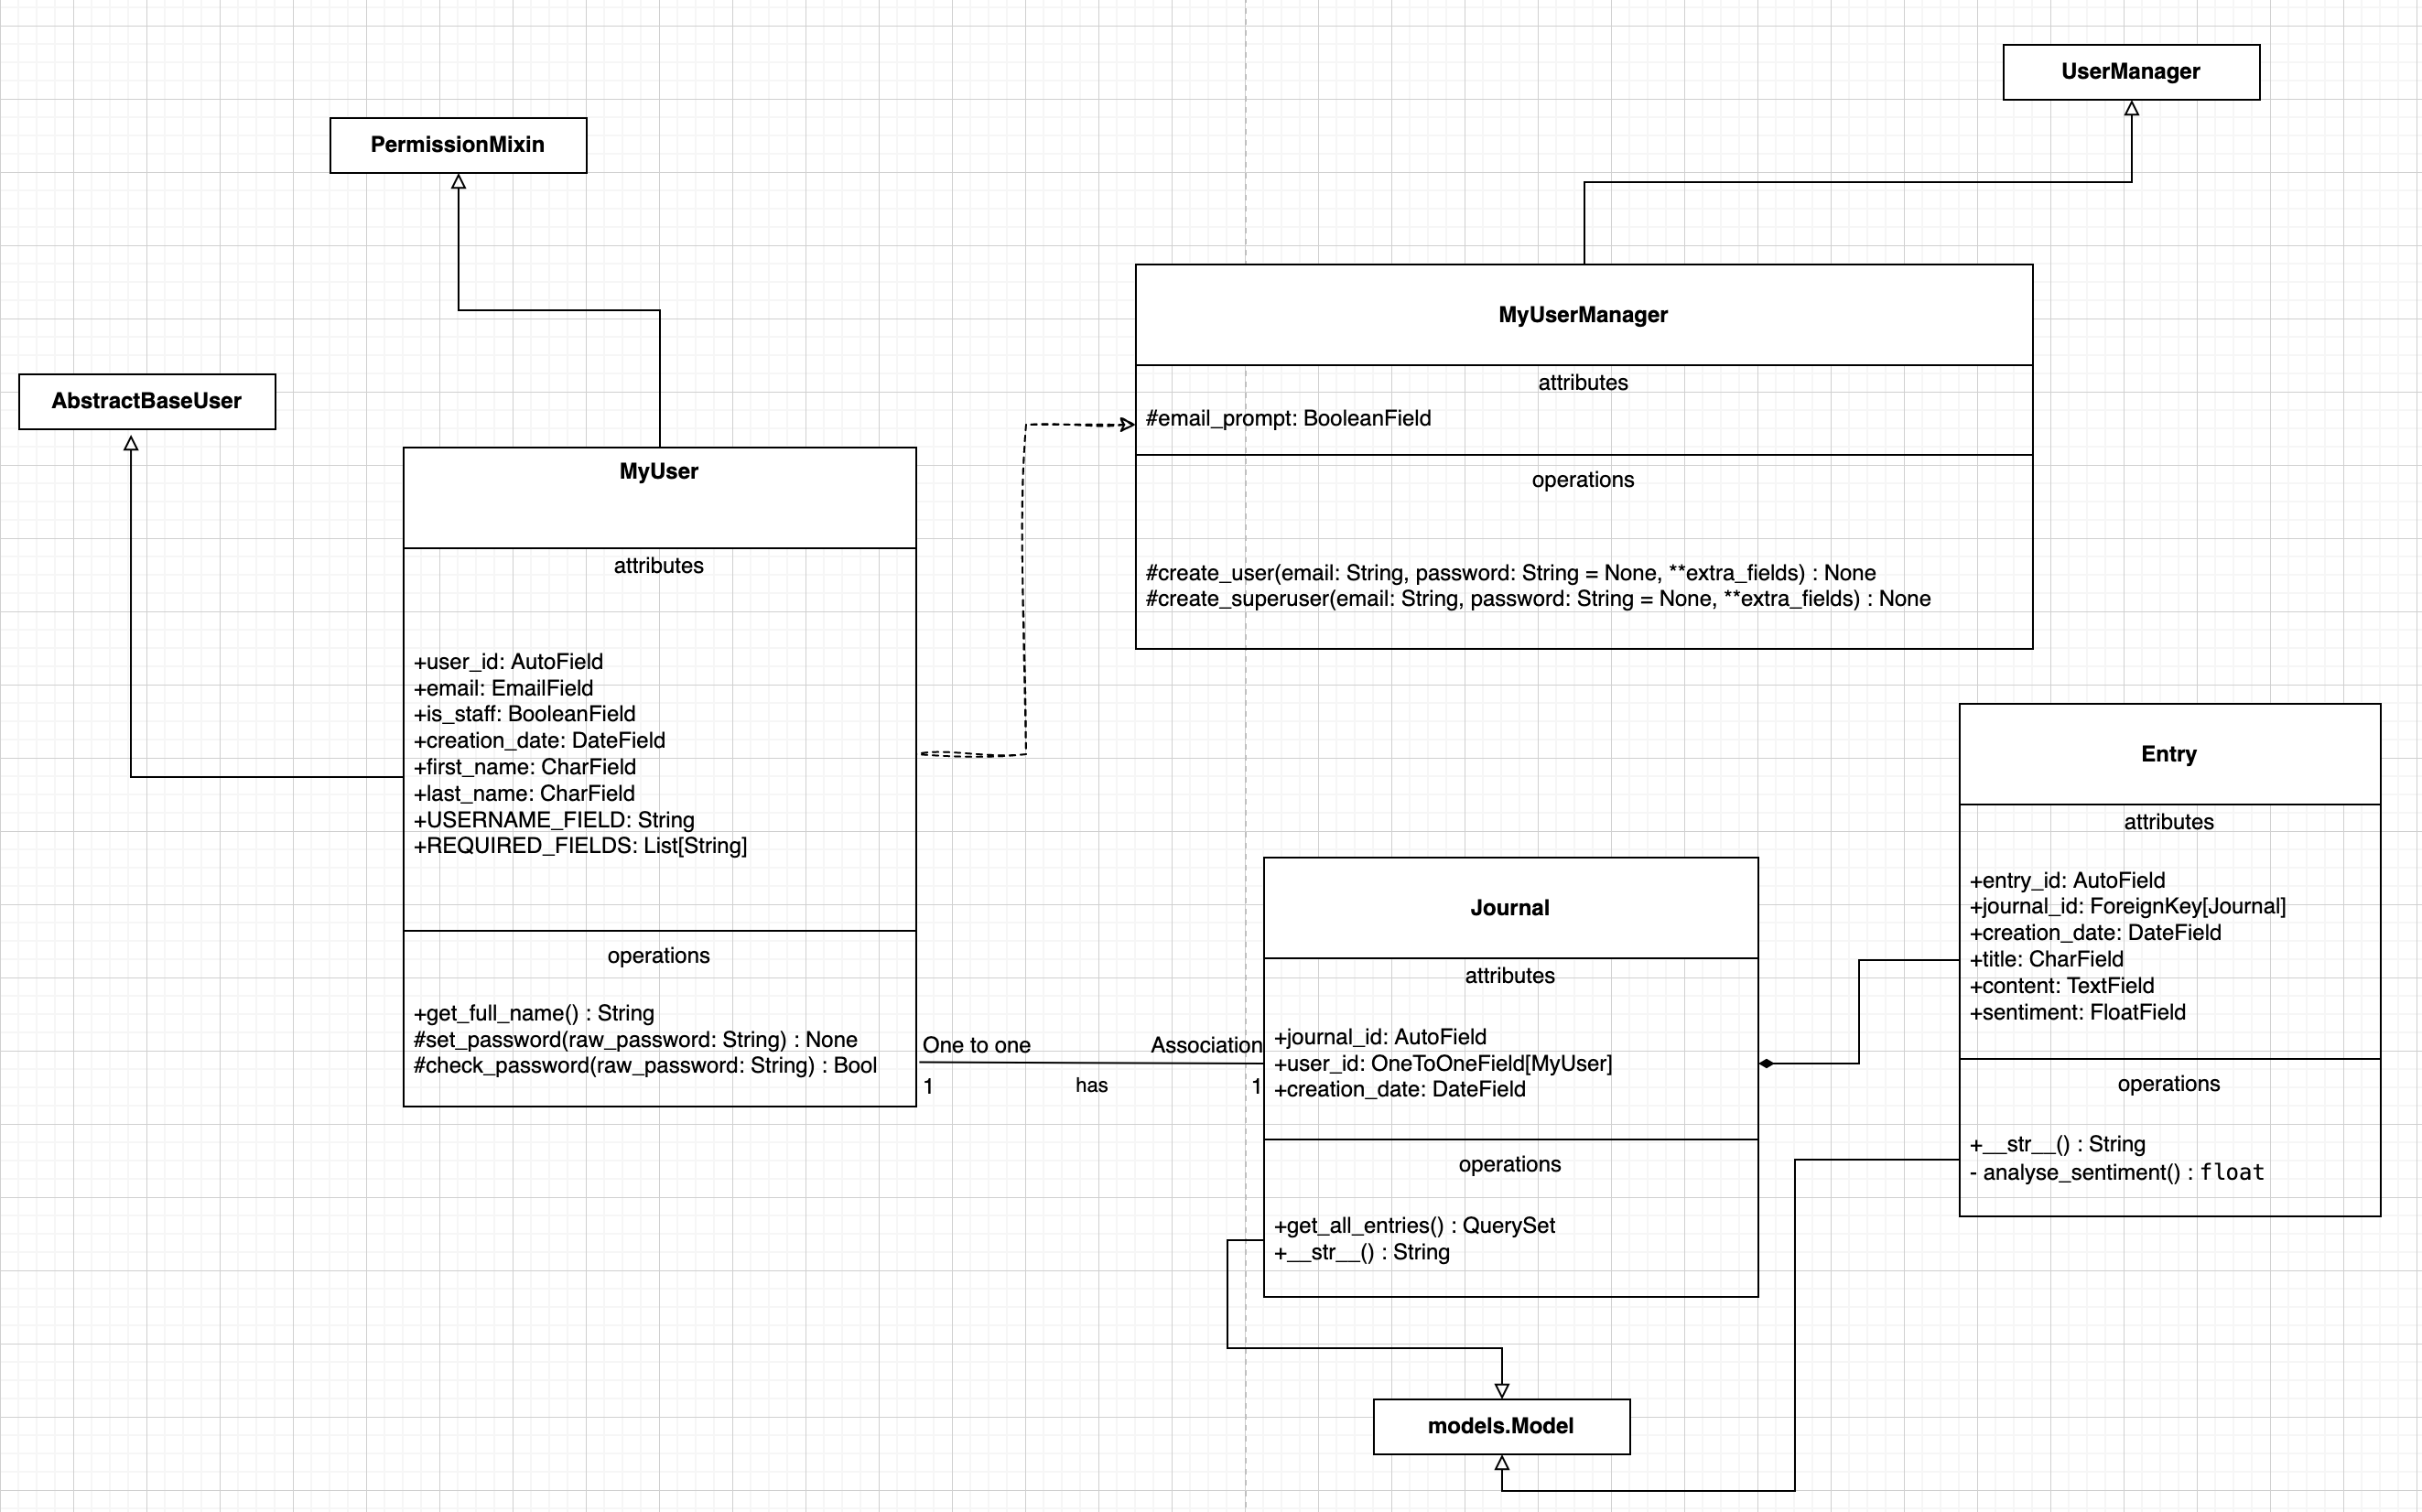
\includegraphics[width=\linewidth]{Assets/UML.png}
    \caption{UML Class Diagram}
    \label{fig:UML}
\end{figure}

In my models.py file, I have defined several classes that represent different objects in my project:

- MyUser: A class which represents my custom user model in Django, with additional fields and methods tailored to my project's requirements. 

- MyUserManager: A class that manages MyUser class objects, including creating new user instances. MyUser has a dependency on MyUserManager for its functionality.

- Journal: A class representing a journal entry in my project, with fields such as title, content, and date. Journal has a one to one association with MyUser class.

- Entry: A class with a composition relationship with the Journal class, representing a single entry within a journal.

Multiple inheritance is a feature that's not common to all OOP languages since it can lead to potential conflicts and ambiguity in the class hierarchy. In Python, it is supported, and as you can see in the UML diagram, MyUser inherits from AbstractBaseUser and PermissionsMixin. An abstract class is a class that acts as a blueprint for creating a new derived class. I have inherited Django's blueprint for creating users, and I have designed my own user class, which depends on the email field for user registration and login. The second inheritance is from the PermissionsMixin class; this enhances my user class with built-in methods for handling user permissions and authorisation, which is useful. 

Both the Journal and Entry classes are inherited from the Django Model class. This allows me to utilise Django's object relational mapping capabilities to interact with the database smoothly. Entry has a composition relationship with a Journal because an entry is a part of a journal and cannot exist independently. Similarly, the Journal class has a one-to-one association with the MyUser class, indicating that each journal entry is associated with a specific user.


\section{File / Table Structures}
Explain the file or table structures used.



\section{Algorithms}
In my frontend application, once all the entries are retrieved from my database, in order to improve the experience of the user, I need there to be a way to sort and filter the entries efficiently. While it is possible to create multiple endpoints in my backend application to return the data in multiple ways (e.g. sorted by date, filtered by category), this can result in unnecessary network requests and slower performance. To optimise the sorting and filtering of entries, I can implement an efficient algorithm in my frontend application.

For my purpose I will implement the sorting based on the entry submission date, although it can easily be modified to include other criteria such as the sentiment of the entries.

Choosing an effective algorithm can improve responsiveness of the application and it can especially do so for long term users of the application who might have a large number of entries in their journal.

Sorting algorithms like bubble sort and insertion sort are bad for large datasets since they have a time complexity of O(\(n^2\)) on average. Hence, I will be choosing an efficient sorting algorithm such as Quicksort or Merge Sort, two divide and conquer algorithms, which have a time complexity of $O(n\log{}n)$ on average. Between the two, both offer good performance but they have different implementations and trade offs. I have chosen Quicksort over merge due to the fact that it is In-Place. This means that copies of the list are not created to sort it, making it more efficient in terms of memory.

Writing my own sorting algorithm gives me greater flexibility as I am able to define what is the key that I am deriving my my entries. In my specific case, I have chosen to implement the QuickSort algorithm for sorting the entries based of the creation date of the entry. 



\section{User Interface}
\subsection{Wireframe Design}

% include figures of wireframe designs which takes up the bulk of the page
\begin{figure}[H]
    \centering
    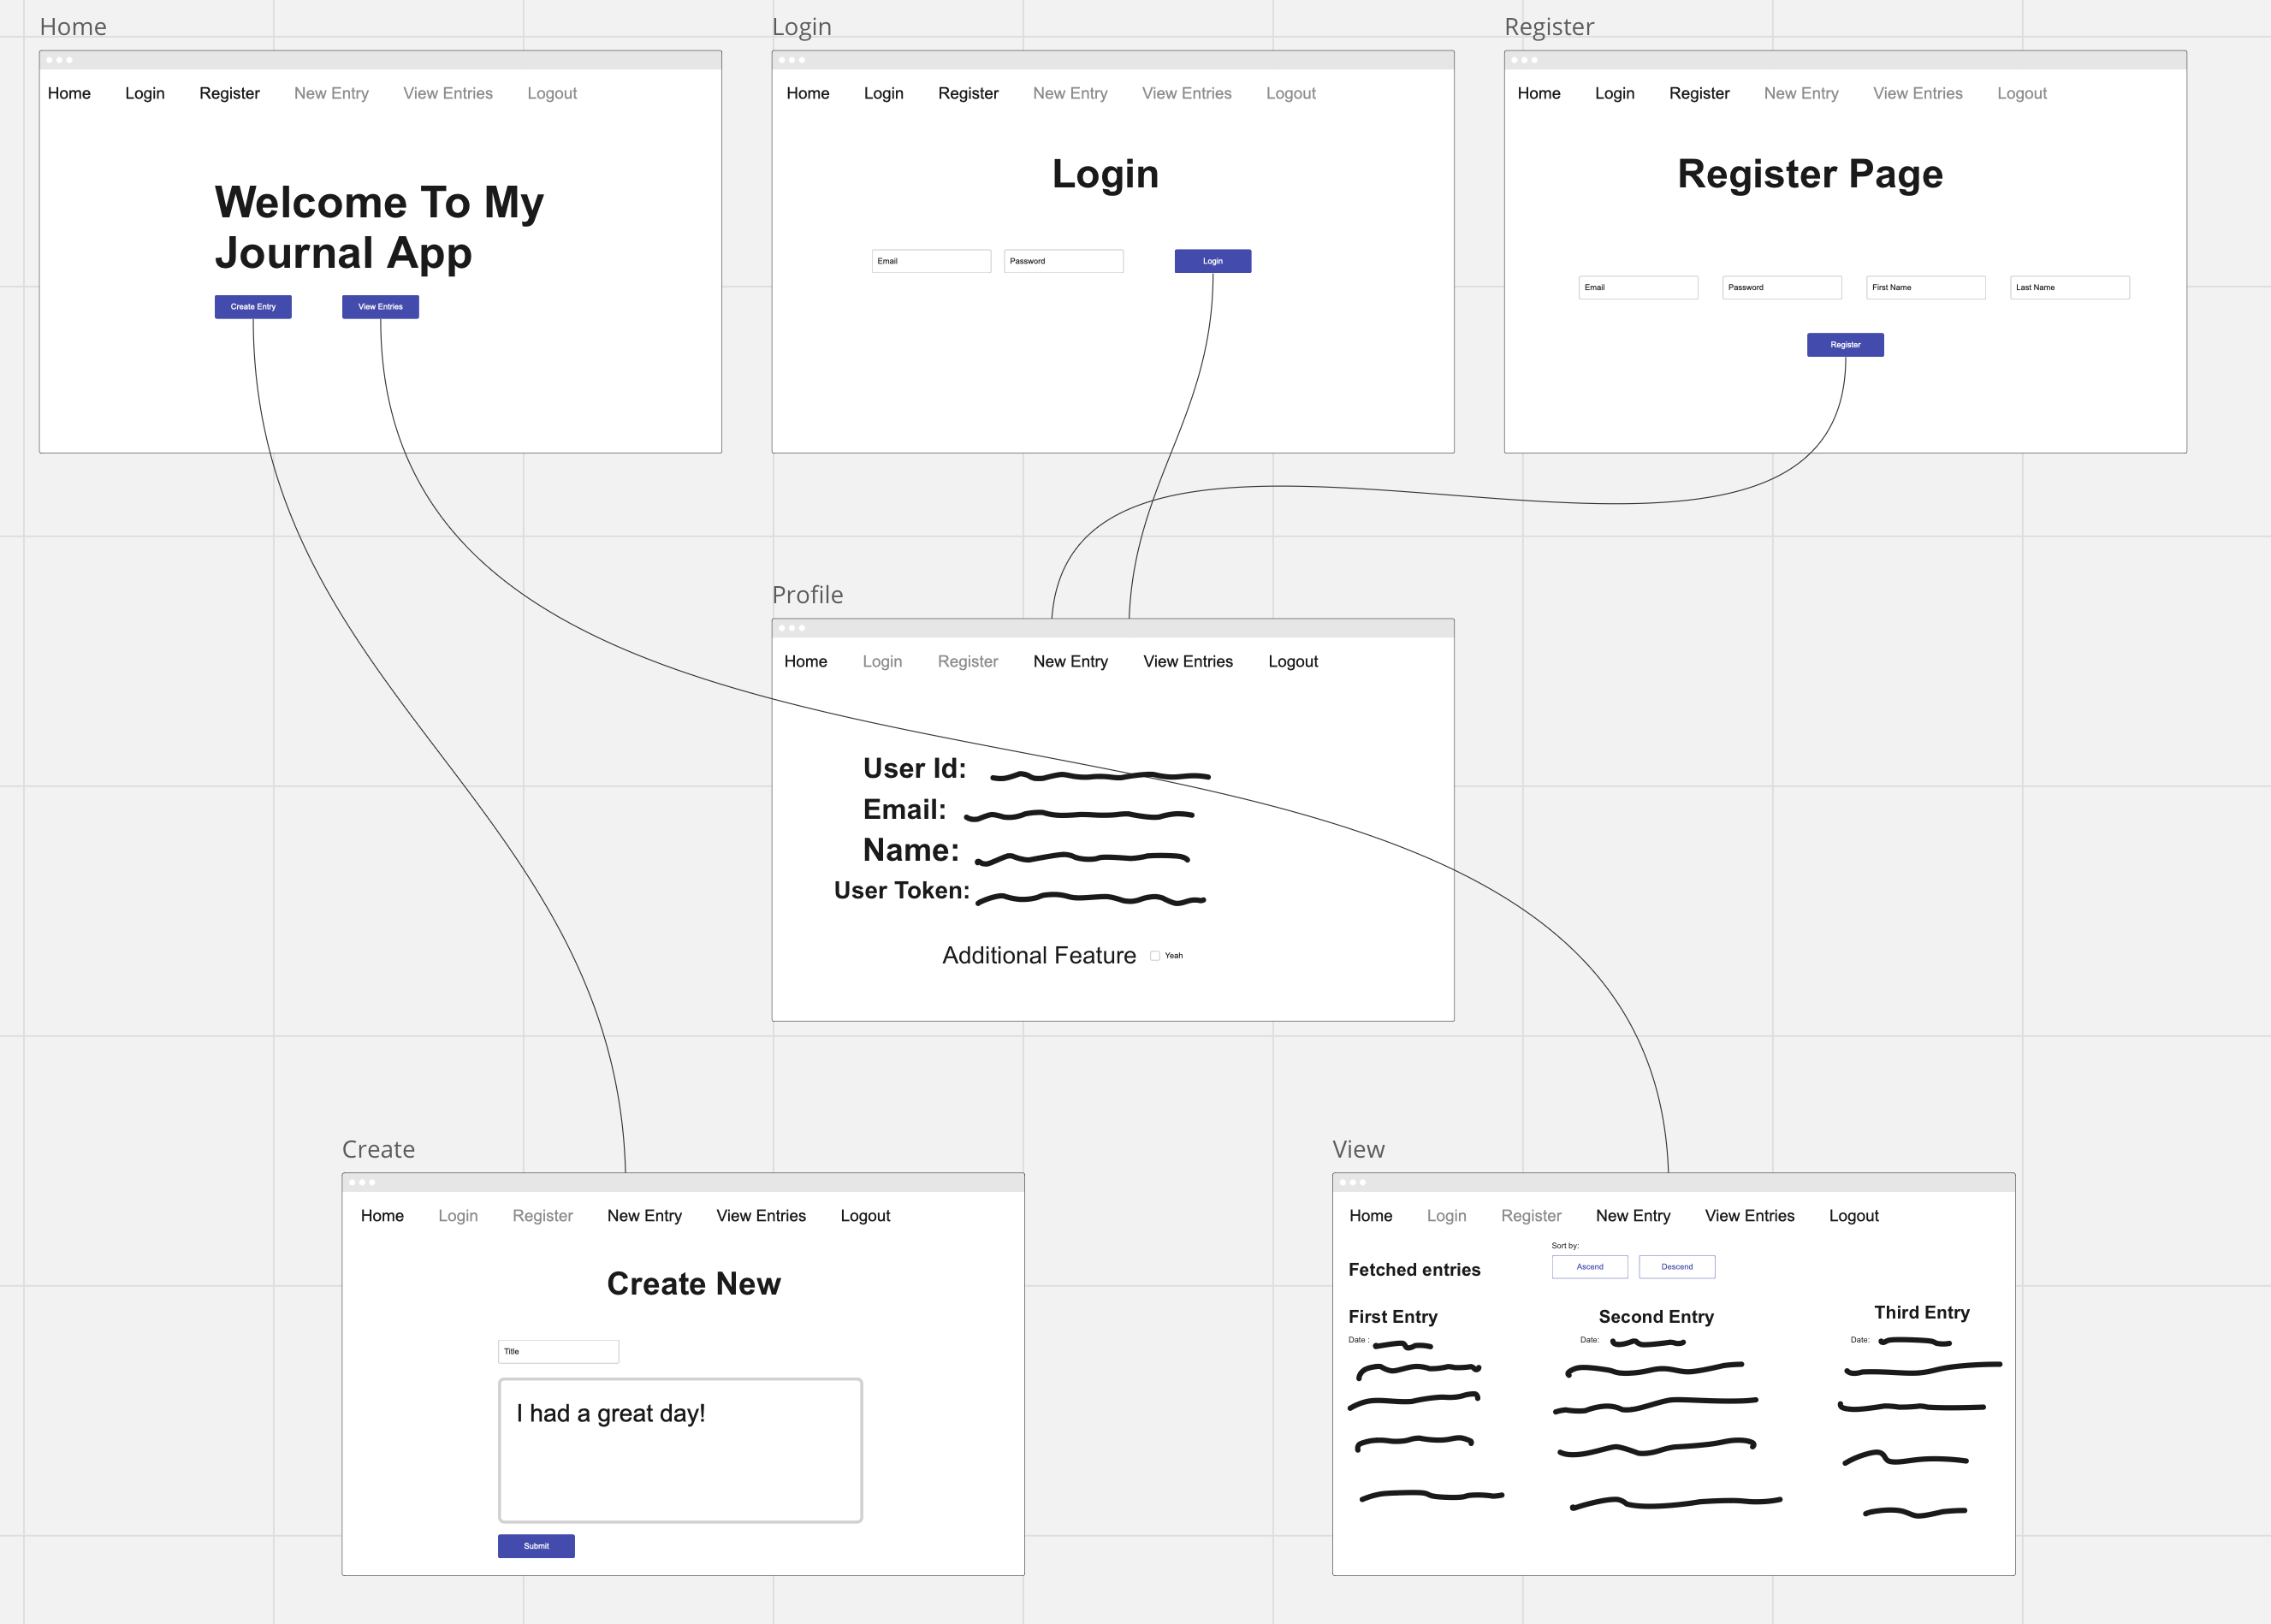
\includegraphics[width=0.8\textwidth]{Assets/all_pages.png}
    \caption{This is an overview of all the screens inside my application, it includes the home page, login page, register page, profile page, create page and view page. There are lines connecting the pages to show the flow of the application. Using the navigation bar at the top, the user can navigate to any page from any page.}
\end{figure}


\begin{figure}[H]
    \centering
    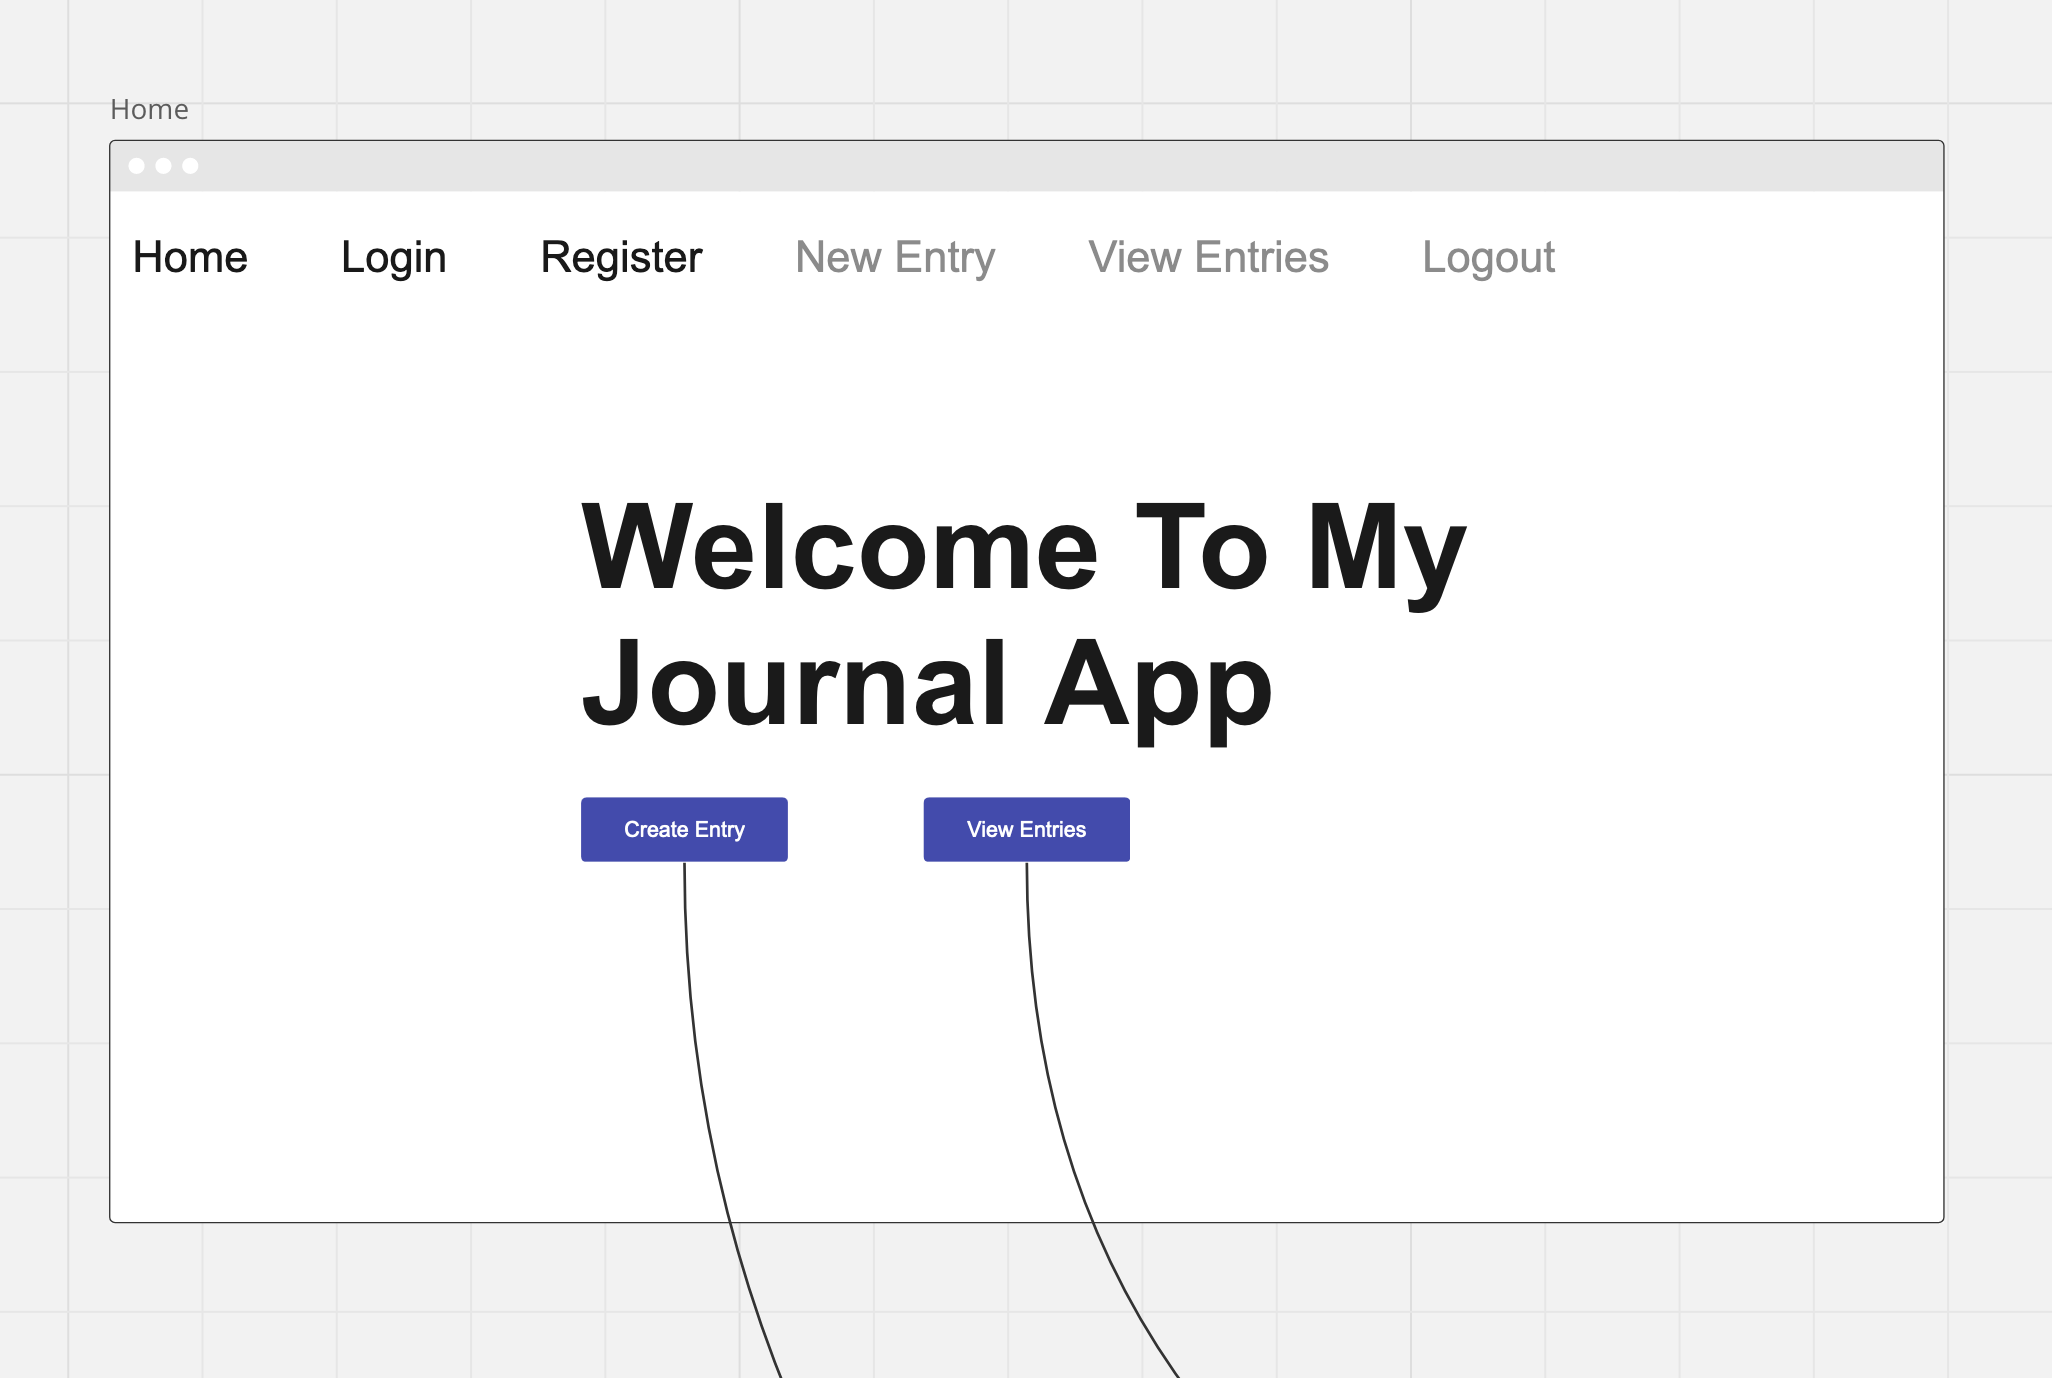
\includegraphics[width=0.7\textwidth]{Assets/home_page.png}
    \caption{The homepage of my application, it includes a navigation bar at the top, a welcome message and buttons for creating and viewing the user's journal entries.}
\end{figure}

\begin{figure}[H]
    \centering
    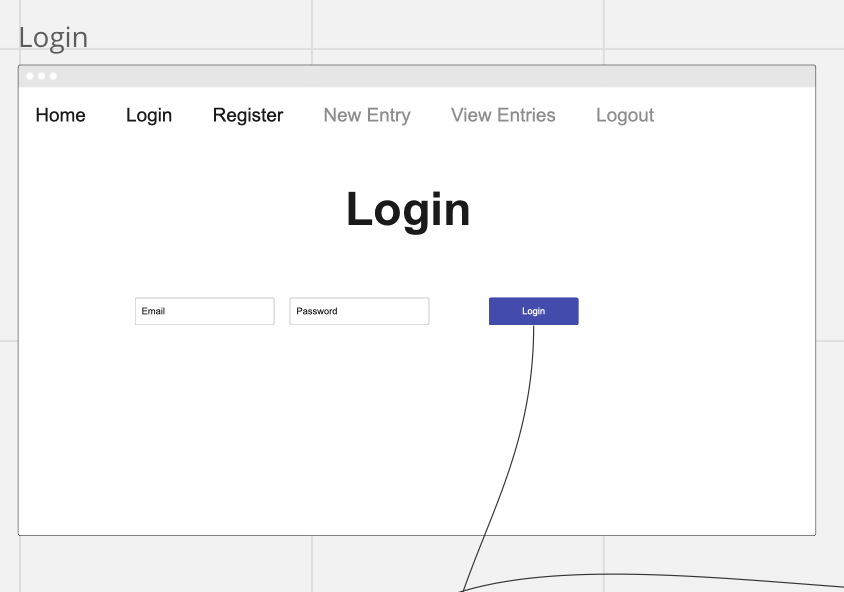
\includegraphics[width=0.7\textwidth]{Assets/login_page.png}
    \caption{The login page of my application, it includes a navigation bar at the top, a form for the user to input their email and password and a button to submit the form. As you can see in the navigation bar, New Entry, View Entries and Logout are all greyed out, this is assuming that the user is not logged in.}
\end{figure}

\begin{figure}[H]
    \centering
    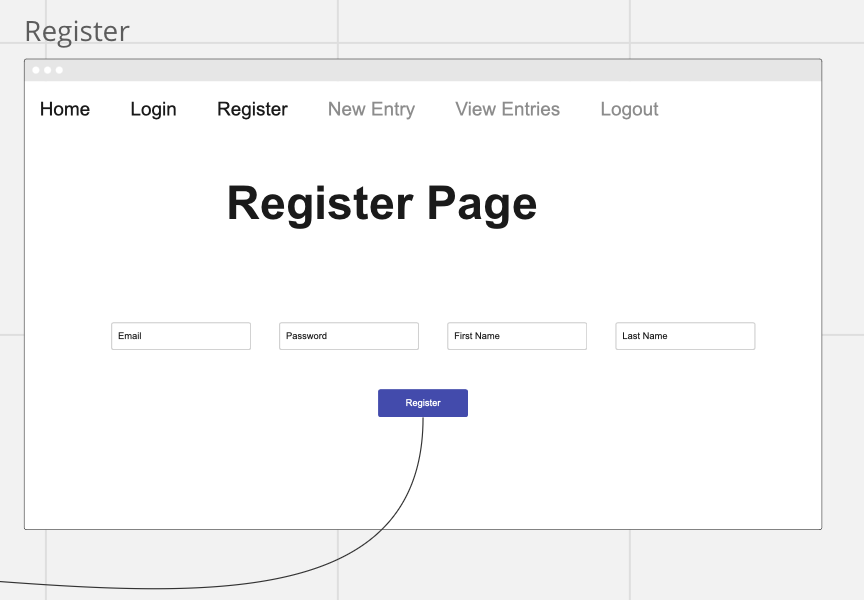
\includegraphics[width=0.8\textwidth]{Assets/register_page.png}
    \caption{Register page is very similar to the login page, it includes a navigation bar at the top, a form for the user inputs as well as the submission button. Registration field requires a couple more fields than the login page.}
\end{figure}

\begin{figure}[H]
    \centering
    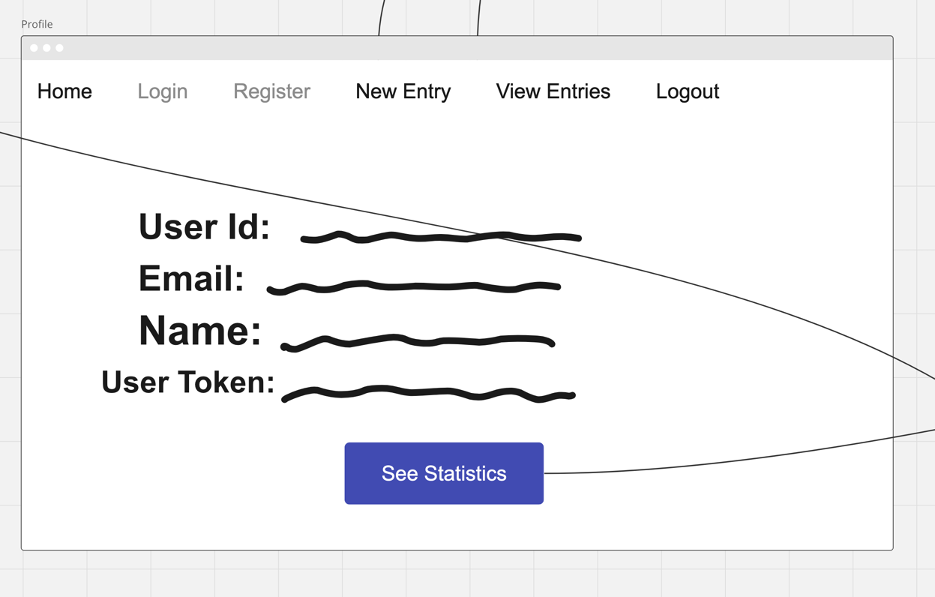
\includegraphics[width=0.8\textwidth]{Assets/profile_page.png}
    \caption{Profile page is where the user can view their profile information, as well as place where they can opt in for some additional features.}
\end{figure}

\begin{figure}[H]
    \centering
    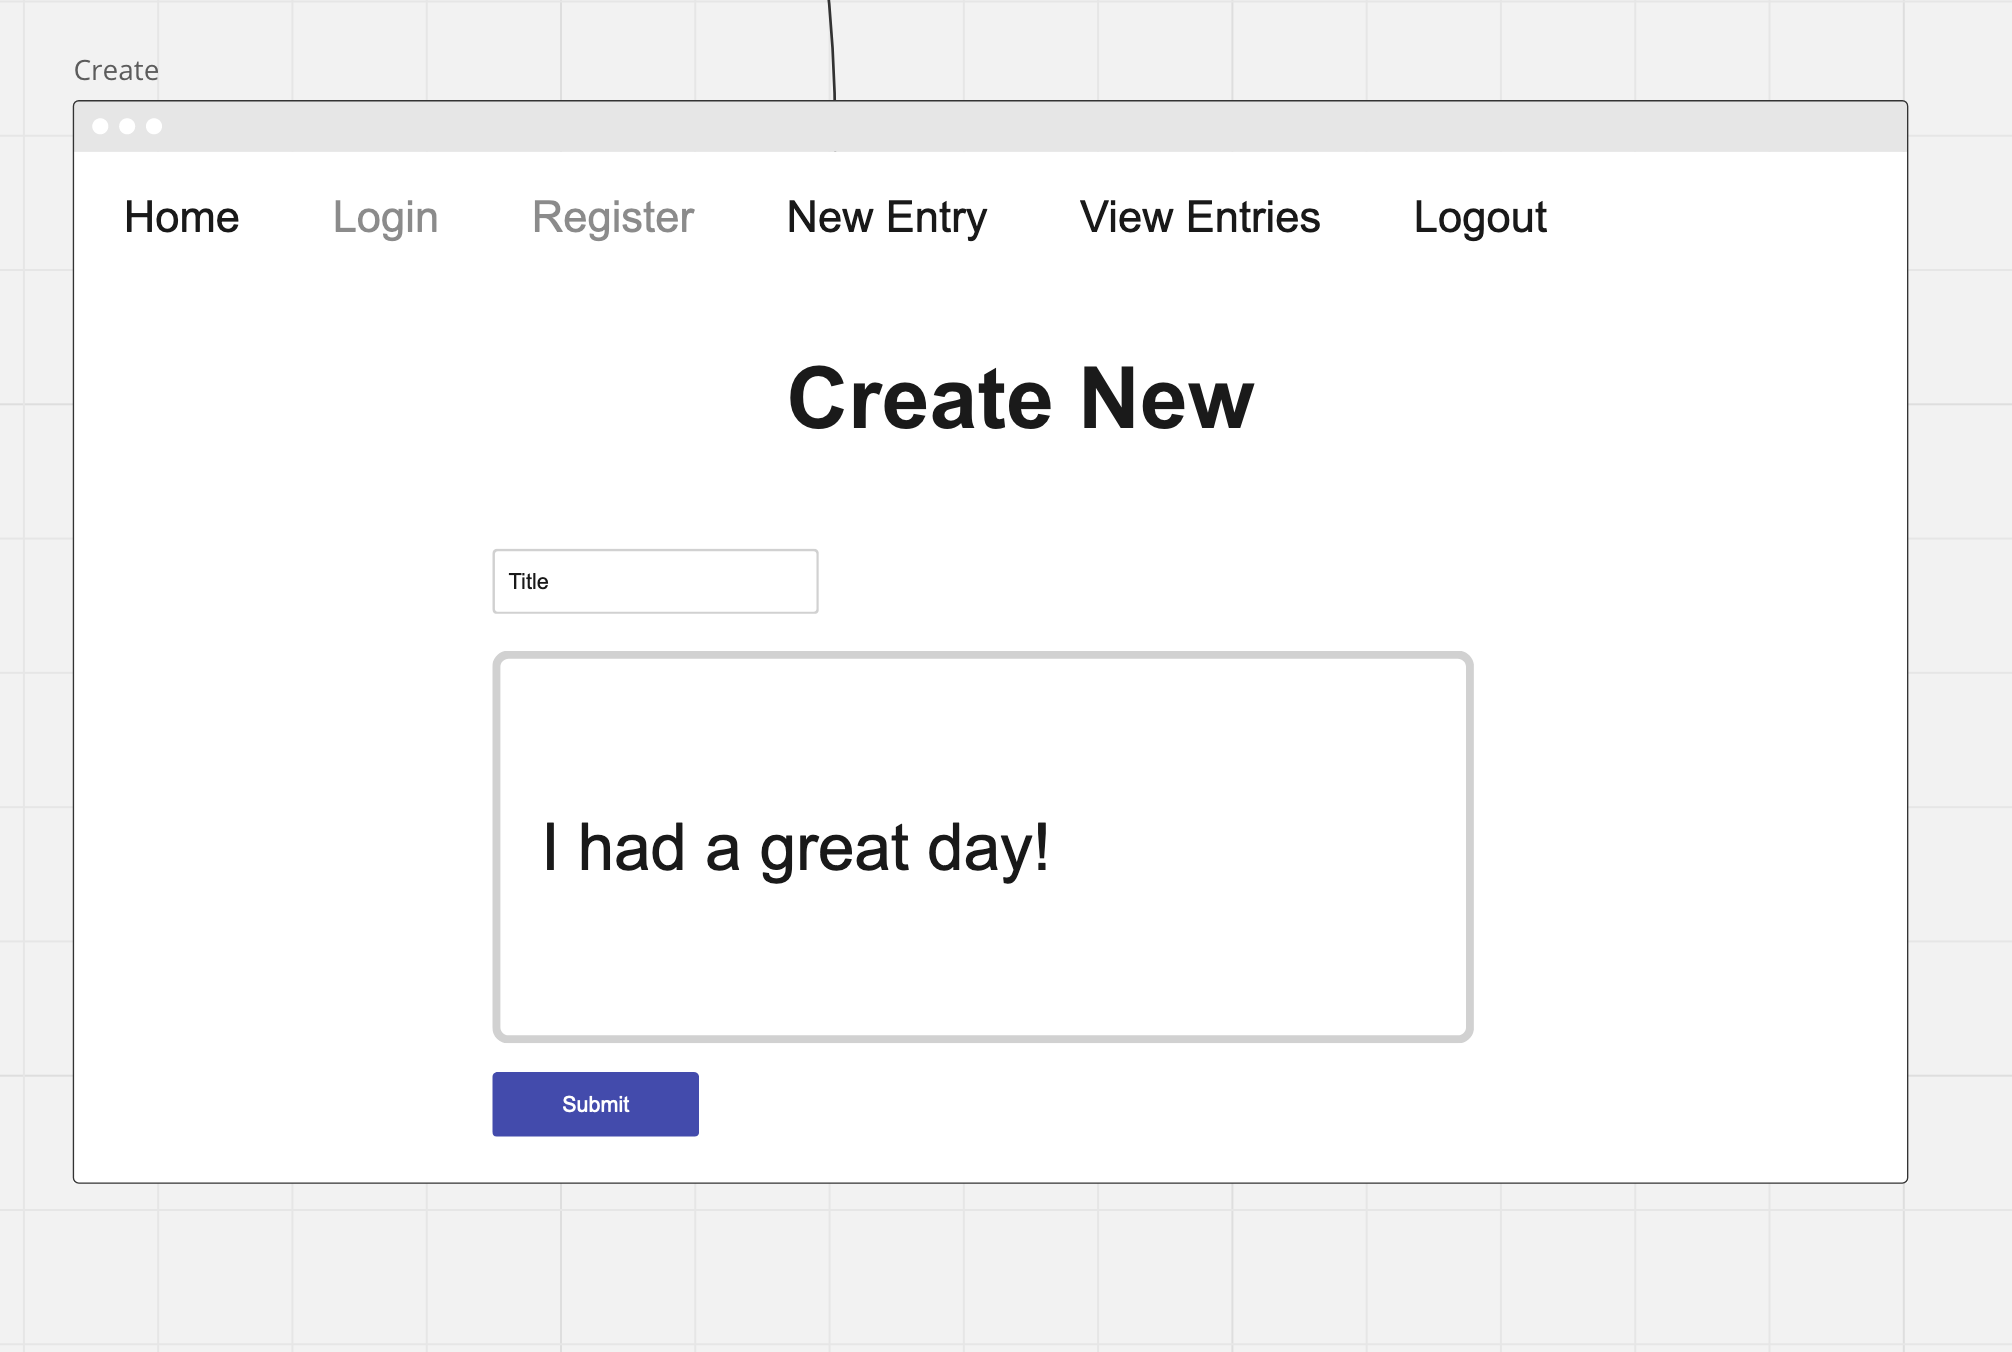
\includegraphics[width=0.8\textwidth]{Assets/create_page.png}
    \caption{Create page is where the user can create a new journal entry. It includes a form for the user to input the title and content of the entry.}
\end{figure}

\begin{figure}[H]
    \centering
    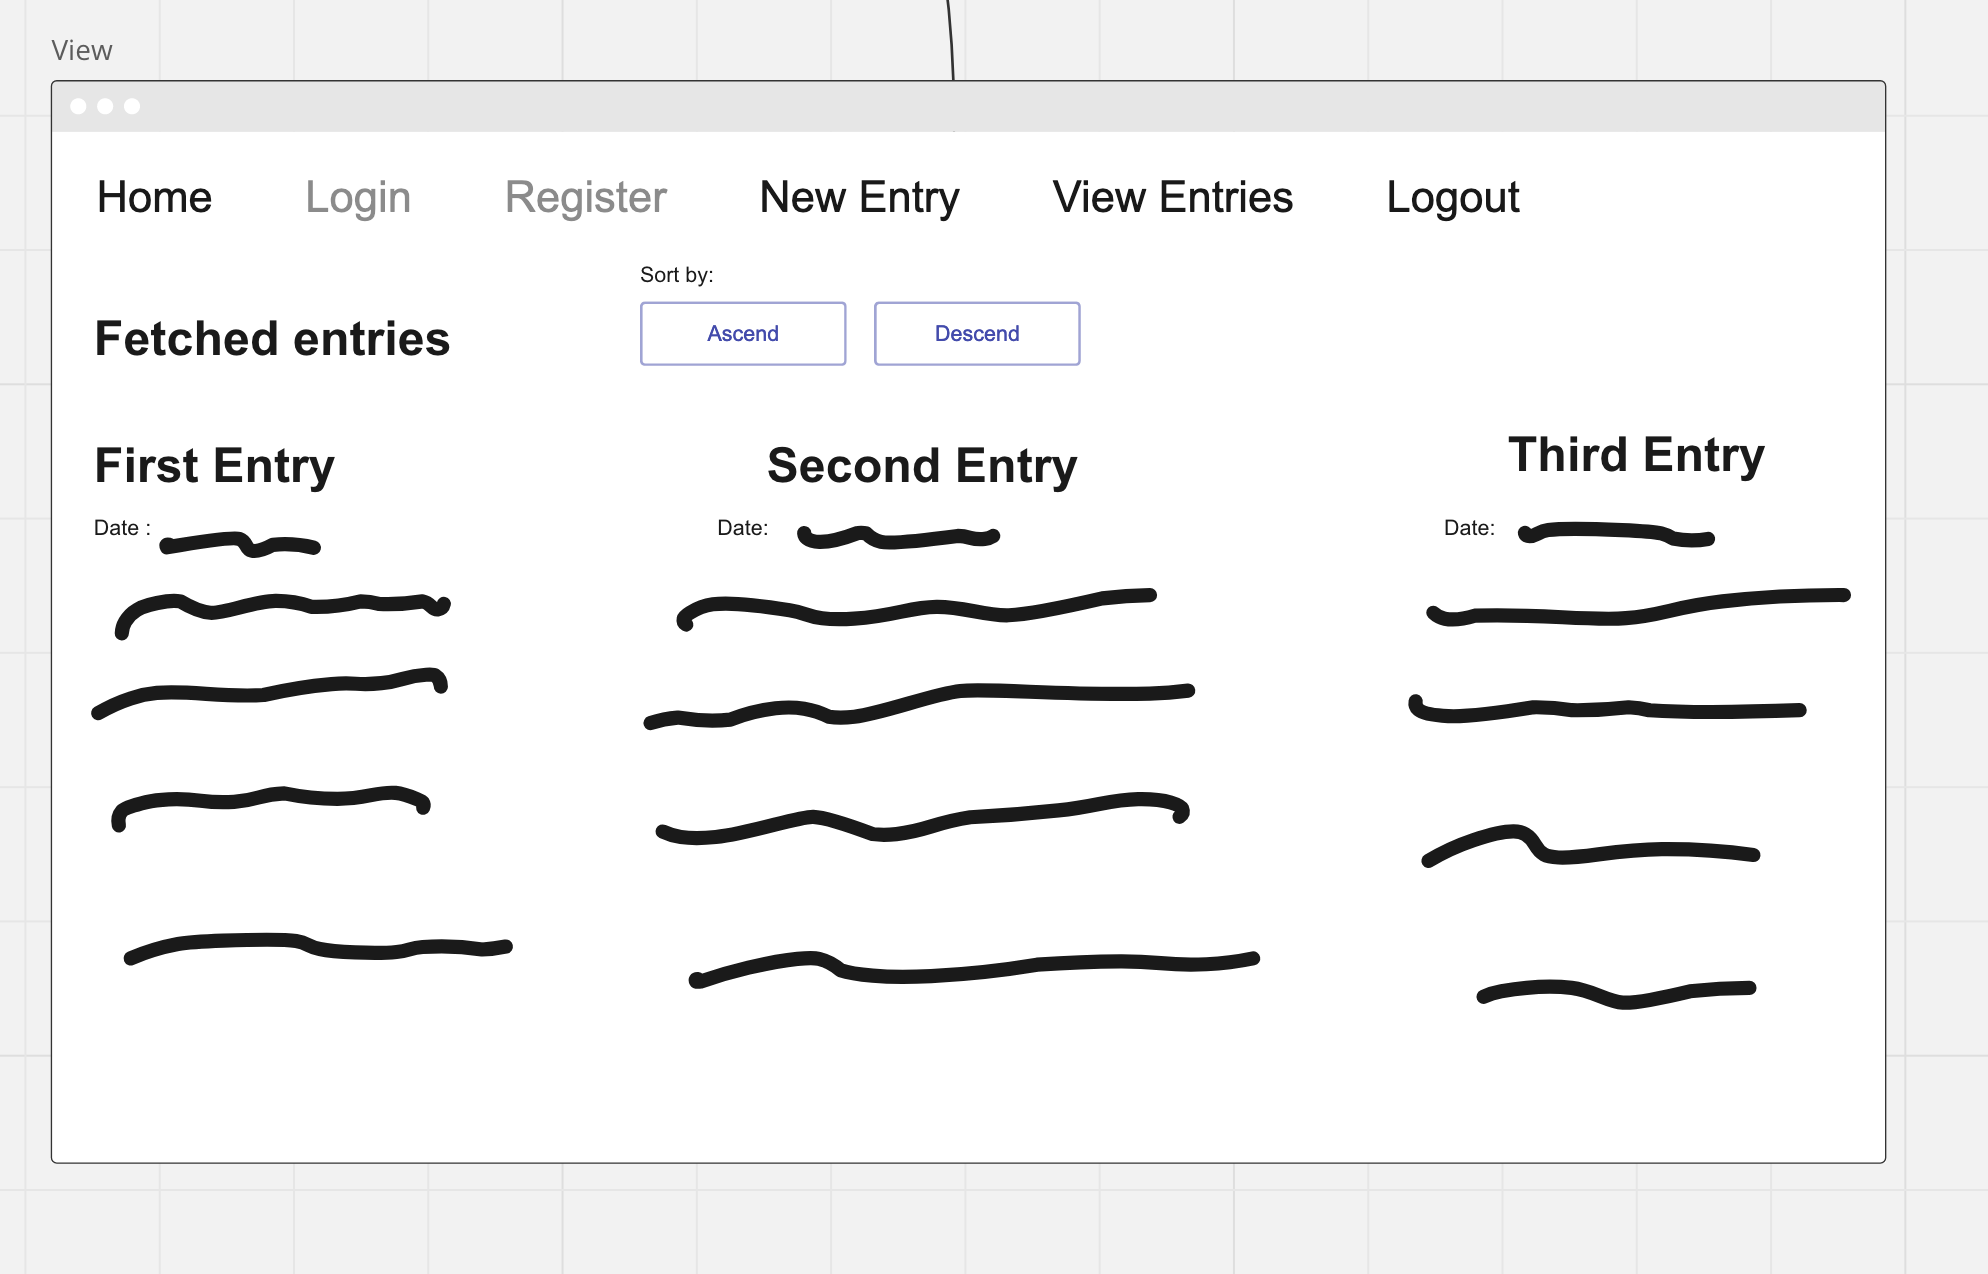
\includegraphics[width=0.8\textwidth]{Assets/view_page.png}
    \caption{View page is where the user can view all of their journal entries. It includes buttons to enable users to sort the entries.}
\end{figure}


\section{RESTful API Endpoints}


\section{Hardware \& Software Requirements}
Specify the hardware and software requirements for the project.

\section{User Authentication}
\subsection{Session Based Authentication}
Session based authentication is where a session is generated and an ID is stored in the Cookie
